%File: anonymous-submission-latex-2024.tex
\documentclass[letterpaper]{article} % DO NOT CHANGE THIS
\usepackage{aaai24}  % DO NOT CHANGE THIS
\usepackage{times}  % DO NOT CHANGE THIS
\usepackage{helvet}  % DO NOT CHANGE THIS
\usepackage{courier}  % DO NOT CHANGE THIS
\usepackage[hyphens]{url}  % DO NOT CHANGE THIS
\usepackage{graphicx} % DO NOT CHANGE THIS
\urlstyle{rm} % DO NOT CHANGE THIS
\def\UrlFont{\rm}  % DO NOT CHANGE THIS
\usepackage{natbib}  % DO NOT CHANGE THIS AND DO NOT ADD ANY OPTIONS TO IT
\usepackage{caption} % DO NOT CHANGE THIS AND DO NOT ADD ANY OPTIONS TO IT
\frenchspacing  % DO NOT CHANGE THIS
\setlength{\pdfpagewidth}{8.5in} % DO NOT CHANGE THIS
\setlength{\pdfpageheight}{11in} % DO NOT CHANGE THIS
%
% These are recommended to typeset algorithms but not required. See the subsubsection on algorithms. Remove them if you don't have algorithms in your paper.
\usepackage{algorithm}
\usepackage{algorithmic}
\usepackage{amsmath}
\usepackage{booktabs}
\usepackage{amsfonts}
\usepackage{array}
\usepackage{multirow}
\usepackage{subcaption}
\usepackage{enumitem}
\usepackage{arydshln}
\usepackage{textpos} 
%
% These are are recommended to typeset listings but not required. See the subsubsection on listing. Remove this block if you don't have listings in your paper.
\usepackage{newfloat}
\usepackage{listings}
\DeclareCaptionStyle{ruled}{labelfont=normalfont,labelsep=colon,strut=off} % DO NOT CHANGE THIS
\lstset{%
	basicstyle={\footnotesize\ttfamily},% footnotesize acceptable for monospace
	numbers=left,numberstyle=\footnotesize,xleftmargin=2em,% show line numbers, remove this entire line if you don't want the numbers.
	aboveskip=0pt,belowskip=0pt,%
	showstringspaces=false,tabsize=2,breaklines=true}
\floatstyle{ruled}
\newfloat{listing}{tb}{lst}{}
\floatname{listing}{Listing}
%
% Keep the \pdfinfo as shown here. There's no need
% for you to add the /Title and /Author tags.
\pdfinfo{
/TemplateVersion (2024.1)
}

% DISALLOWED PACKAGES
% \usepackage{authblk} -- This package is specifically forbidden
% \usepackage{balance} -- This package is specifically forbidden
% \usepackage{color (if used in text)
% \usepackage{CJK} -- This package is specifically forbidden
% \usepackage{float} -- This package is specifically forbidden
% \usepackage{flushend} -- This package is specifically forbidden
% \usepackage{fontenc} -- This package is specifically forbidden
% \usepackage{fullpage} -- This package is specifically forbidden
% \usepackage{geometry} -- This package is specifically forbidden
% \usepackage{grffile} -- This package is specifically forbidden
% \usepackage{hyperref} -- This package is specifically forbidden
% \usepackage{navigator} -- This package is specifically forbidden
% (or any other package that embeds links such as navigator or hyperref)
% \indentfirst} -- This package is specifically forbidden
% \layout} -- This package is specifically forbidden
% \multicol} -- This package is specifically forbidden
% \nameref} -- This package is specifically forbidden
% \usepackage{savetrees} -- This package is specifically forbidden
% \usepackage{setspace} -- This package is specifically forbidden
% \usepackage{stfloats} -- This package is specifically forbidden
% \usepackage{tabu} -- This package is specifically forbidden
% \usepackage{titlesec} -- This package is specifically forbidden
% \usepackage{tocbibind} -- This package is specifically forbidden
% \usepackage{ulem} -- This package is specifically forbidden
% \usepackage{wrapfig} -- This package is specifically forbidden
% DISALLOWED COMMANDS
% \nocopyright -- Your paper will not be published if you use this command
% \addtolength -- This command may not be used
% \balance -- This command may not be used
% \baselinestretch -- Your paper will not be published if you use this command
% \clearpage -- No page breaks of any kind may be used for the final version of your paper
% \columnsep -- This command may not be used
% \newpage -- No page breaks of any kind may be used for the final version of your paper
% \pagebreak -- No page breaks of any kind may be used for the final version of your paperr
% \pagestyle -- This command may not be used
% \tiny -- This is not an acceptable font size.
% \vspace{- -- No negative value may be used in proximity of a caption, figure, table, section, subsection, subsubsection, or reference
% \vskip{- -- No negative value may be used to alter spacing above or below a caption, figure, table, section, subsection, subsubsection, or reference

\setcounter{secnumdepth}{2} %May be changed to 1 or 2 if section numbers are desired.

% The file aaai24.sty is the style file for AAAI Press
% proceedings, working notes, and technical reports.
%

% Title

% Your title must be in mixed case, not sentence case.
% That means all verbs (including short verbs like be, is, using,and go),
% nouns, adverbs, adjectives should be capitalized, including both words in hyphenated terms, while
% articles, conjunctions, and prepositions are lower case unless they
% directly follow a colon or long dash
\title{An Empirical Study of CLIP for Text-based Person Search}
\author{
    %Authors
    % All authors must be in the same font size and format.
    Min Cao\textsuperscript{\rm 1},
    Yang Bai\textsuperscript{\rm 1},
    Ziyin Zeng\textsuperscript{\rm 1},
    Mang Ye\textsuperscript{\rm 2},
    Min Zhang\textsuperscript{\rm 1}
}
\affiliations{
    \textsuperscript{\rm 1}School of Computer Science and Technology, Soochow University\\
    \textsuperscript{\rm 2}School of Computer Science, Wuhan University
    % \textsuperscript{\rm 3}Harbin Institute of Technology, Shenzhen
%
% See more examples next
}

%Example, Single Author, ->> remove \iffalse,\fi and place them surrounding AAAI title to use it
\iffalse
\title{My Publication Title --- Single Author}
\author {
    Author Name
}
\affiliations{
    Affiliation\\
    Affiliation Line 2\\
    name@example.com
}
\fi

\iffalse
%Example, Multiple Authors, ->> remove \iffalse,\fi and place them surrounding AAAI title to use it
\title{My Publication Title --- Multiple Authors}
\author {
    % Authors
    First Author Name\textsuperscript{\rm 1},
    Second Author Name\textsuperscript{\rm 2},
    Third Author Name\textsuperscript{\rm 1}
}
\affiliations {
    % Affiliations
    \textsuperscript{\rm 1}Affiliation 1\\
    \textsuperscript{\rm 2}Affiliation 2\\
    firstAuthor@affiliation1.com, secondAuthor@affilation2.com, thirdAuthor@affiliation1.com
}
\fi


% REMOVE THIS: bibentry
% This is only needed to show inline citations in the guidelines document. You should not need it and can safely delete it.
\usepackage{bibentry}
% END REMOVE bibentry

\begin{document}

\maketitle

\begin{abstract}
Text-based Person Search (TBPS) aims to retrieve the person images using natural language descriptions. 
Recently, Contrastive Language Image Pretraining (CLIP), a universal large cross-modal vision-language pre-training model, has remarkably performed over various cross-modal downstream tasks due to its powerful cross-modal semantic learning capacity. TPBS, as a fine-grained cross-modal retrieval task, is also facing the rise of research on the CLIP-based TBPS. 
In order to explore the potential of the visual-language pre-training model for downstream TBPS tasks, this paper makes the first attempt to conduct a comprehensive empirical study of CLIP for TBPS and thus contribute a straightforward, incremental, yet strong TBPS-CLIP baseline to the TBPS community.
We revisit critical design considerations under CLIP, including data augmentation and loss function.
The model, with the aforementioned designs and practical training tricks, can attain satisfactory performance \textbf{without any sophisticated modules}. Also, we conduct the probing experiments of TBPS-CLIP in model generalization and model compression, demonstrating the effectiveness of TBPS-CLIP from various aspects.
This work is expected to provide empirical insights and highlight future CLIP-based TBPS research.

% Text-based Person Search (TBPS) aims to retrieve person images using natural language descriptions and is a fine-grained. Recently, Contrastive Language Image Pretraining (CLIP), a cross-modal pre-trained model, has remarkably performed over various cross-modal downstream tasks due to its powerful cross-modal semantic learning capacity. TPBS, as a fine-grained cross-modal retrieval task, is also facing the rise of research on the CLIP-based TBPS. Rather than presenting a novel method by designing sophisticated modules into CLIP for pursuing state-of-the-art results in other methods, this paper conducts a comprehensive empirical study of CLIP for TBPS. It thus contributes a straightforward, incremental, yet strong TBPS-CLIP baseline to the TBPS community. We revisit critical design considerations under CLIP, including data augmentation and loss function. The model, with the aforementioned designs and practical training tricks, can attain satisfactory performance \textbf{without any sophisticated modules}. Also, we conduct the probing experiments of TBPS-CLIP in model generalization, model compression, and few-shot learning. The effectiveness of TBPS-CLIP is demonstrated from various aspects. This work is expected to provide empirical insights and highlight future CLIP-based TBPS research.

%Text-based Person Search (TBPS) aims to retrieve person images using natural language descriptions. Most existing methods typically employ the prior knowledge from the unimodal pre-trained model to facilitate TBPS, which lacks the efficient utilization of cross-modal correspondence information.
%with a lack of cross-modal correspondence information.
% Recently, Contrastive Language Image Pretraining (CLIP), a cross-modal pre-trained model, has remarkably performed over various cross-modal downstream tasks due to its powerful cross-modal semantic learning capacity. In this paper, we conduct a comprehensive empirical study to explore the potential of CLIP for TBPS and revisit critical design considerations, including data augmentation and loss function. We show that the model with the aforementioned designs as well as the effective training tricks, can attain new state-of-the-art results \textbf{without introducing sophisticated modules}, \emph{i.e.}, $73.85\%$, $65.01\%$ and $62.85\%$ Rank-1 accuracy on CUHK-PEDES, ICFG-PEDES and RSTPReid, respectively. Moreover, we provide insight into the internal properties of the model by investigating the contribution of each component to the model, and make a preliminary exploration of the zero/few-shot capability of CLIP for TBPS. We expect this work to provide valuable empirical evidence and insights for future CLIP-based TBPS research.
\end{abstract}

\begin{textblock*}{.8\textwidth}[.5,0](0.5\textwidth, -.560\textwidth)
\centering
{\small Code: \url{https://github.com/Flame-Chasers/TBPS-CLIP}}
\end{textblock*}

\section{Introduction}

Text-based Person Search (TBPS) retrieves the corresponding person images from a large-scale image database given a textual description. 
The task is gradually gaining extensive attention~\cite{jiang2023cross,bai2023rasa} due to its potential applications in searching for suspects, locating lost children, \emph{etc}. 
As a fine-grained retrieval task, TBPS requires the ability to achieve effective cross-modal alignment and efficient cross-modal retrieval for practical applications, both of which bring challenges.

For replying to these challenges, many methods~\cite{zhang2018deep, ding2021semantically, zhao2021weakly} focus on projecting representations extracted from each modality into one shared space.
However, most of them only utilize unimodal pre-trained models as the backbones (\emph{e.g.}, LSTM or BERT for the text encoder, Resnet-50 or ViT for the image encoder), and ignore the powerful Vision-Language Pre-training (VLP) models equipped with an adequate understanding of cross-modal alignment.
In recent years, VLP methods~\cite{lu2019vilbert, li2022blip} have demonstrated remarkable performance on various cross-modal downstream tasks, including visual question answering, image captioning, image-text retrieval, \emph{etc}. Consequently, it has become the dominant paradigm for solving these tasks. 
Considering that the research under VLP for TBPS~\cite{bai2023text,bai2023rasa} is now in its infancy, this paper aims to fully exploit the potential of VLP for TBPS.

\begin{figure}[t]
\setlength{\abovecaptionskip}{0.05cm}
\centerline{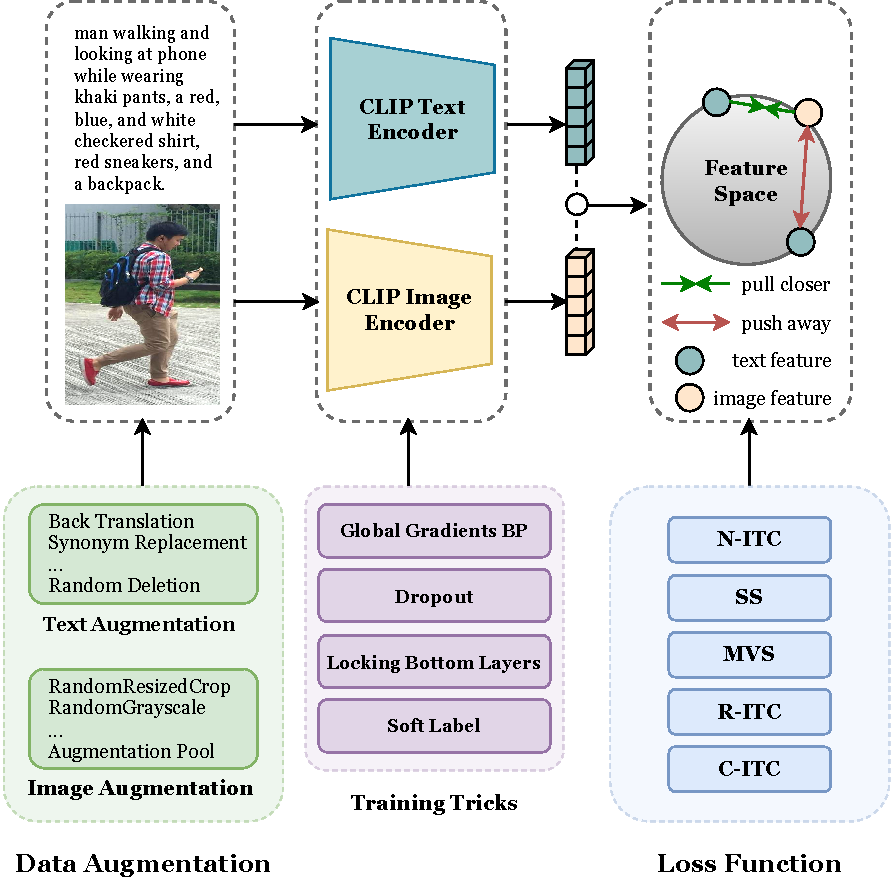
\includegraphics[width=0.75\linewidth,height=0.8\linewidth]{figures/figure1.pdf}}
\caption{Overview of the empirical study on CLIP.} \label{fig:head}
% \caption{Overview of the proposed TBPS-CLIP. The image and text are first augmented through data augmentation. After applied with data augmentation, the two images and one caption are encoded through an image encoder and a text encoder, respectively, to generate the corresponding representations. The distance between the two image representations are minimized by a self-supervision (SS) loss. Each image representation is } \label{fig:head}
\vspace{-0.5cm}
\end{figure}

Among VLP methods, CLIP~\cite{radford2021learning} is one of the most prominent representatives and has demonstrated impressive performance on various downstream tasks~\cite{wang2022cris, wang2022clip}.
In addition, CLIP has the benefit of efficient retrieval due to its independent encoding for each modality. 
These inspire some researchers to explore CLIP-based TBPS methods~\cite{wang2023exploiting, jiang2023cross}.
They specialize in incorporating sophisticated modules into CLIP to enhance performance, lacking the full exploitation of CLIP's pre-trained knowledge and the full utilization of its powerful cross-modal semantic learning capacity.
This paper returns to the origin of CLIP and probes the potential of CLIP tuning for TBPS. 
For this, we conduct a comprehensive empirical study of CLIP for TBPS from two aspects: data augmentation and loss function. 

1) Data augmentation.
It is a prevalent and effective technique to increase the generalization of models by learning augmentation-invariant representations between the original input and the augmented version. 
% Until now, there have been no TBPS methods to deeply explore this technique, replaced by usually a simple utilization of random horizontal flip for the image and nothing for other data (\emph{i.e.}, text and image-text pair)~\cite{wang2020vitaa, chen2022tipcb, ding2021semantically}.
Until now, none of the TBPS methods have deeply and systematically explored this technique. Instead, they typically employ a simple utilization of random horizontal flip for the image while not applying any augmentation to the text~\cite{wang2020vitaa, chen2022tipcb, ding2021semantically}.
In this study, we comprehensively evaluate various data augmentation strategies, thereby deriving a powerful data augmentation strategy for TBPS.

2) Loss function.
% The current model is generally equipped with pretext tasks for representation learning.
Designing rational and practical loss functions is critical to improving performance and has been an increasingly active research direction in TBPS community~\cite{zhang2018deep, bai2023rasa}.
We take CLIP as a hotbed and conduct a series of probing studies to analyze the effectiveness of various loss functions in TBPS.
Unlike the loss functions in existing TBPS methods that are well-designed mainly from exploring the TBPS task and belong to the task-oriented loss functions, the loss functions probed in this study are primarily inspired by VLP communities and are pretty generic to various cross-modal tasks.

These empirical studies above, combined with other valuable tricks detailed in later sections, enable us to develop a strong TBPS-CLIP baseline.
\textbf{Unlike other methods of designing sophisticated modules, TBPS-CLIP attains competitive performance under a very lightweight and low-cost architecture, in which merely several common training tricks, data augmentations and loss functions are added into CLIP.}
%\textbf{By merely incorporating common training tricks, data augmentations and loss functions into CLIP, TBPS-CLIP achieves competitive performance without designing sophisticated modules, unlike other methods.}
% Taking a step further, we also provide insights into the internal properties and functionalities of TBPS-CLIP, by which we investigate the contribution of each component in TBPS-CLIP to the final retrieval performance by two evaluation metrics.
In order to fully demonstrate the effectiveness and generalization of TBPS-CLIP, we further develop some valuable additional probing experiments.

1) Model generalization.
For one thing, CLIP has become a baseline of various tasks due to its effectiveness and simplicity, likewise, TBPS-CLIP is targeted as the baseline of TBPS, for which its effectiveness as the baseline is experimentally proved. 
For another thing, beyond only employing CLIP for the supervised TBPS, we provide a preliminary exploration of the few-shot TBPS under CLIP and the superiority of TBPS-CLIP in the few-shot setting is also proved.

2) Model compression. 
We provide insights into the internal properties of TBPS-CLIP by investigating the contribution of each module to the final retrieval performance. These insights offer the guidance for compression of TBPS-CLIP.

%3) Few-shot learning.
%CLIP and its variants~\cite{zhou2022learning} have provided a promising solution for some cross-modal tasks in the few-shot setting. Inspired by them, beyond only employing CLIP to perform the supervised TBPS, this paper provides a preliminary exploration of the few-shot TBPS based on CLIP. Most crucially, the superiority of TBPS-CLIP under the few-shot setting is also proved.

In summary, this paper mainly contributes a strong TBPS-CLIP baseline to the TBPS community.
TBPS-CLIP has features of high-performance, lightweight and low-cost architecture and ease of use.
Besides these, we show its advantage in model generalization and model compression.
All these manifest the applicability of TBPS-CLIP in both the academy and industry.
Lots of experiments are expected to provide empirical insights for future research.



%Furthermore, we also provide insights into the internal properties and functionalities of TBPS-CLIP by investigating the contribution of each component to the final retrieval performance, using two evaluation metrics. These insights are expected to offer guidance for model compression and pruning in real-world applications.
%Finally, we have noticed that CLIP and its variants~\cite{zhou2022learning,gao2021clip} have provided a promising solution for some cross-modal downstream tasks under the zero-shot and few-shot settings.
%Inspired by them, beyond only employing CLIP as a benchmark to perform the fully supervised TBPS, this paper provides a preliminary exploration of the zero/few-shot TBPS based on CLIP.


\section{Related Work}
\subsection{Text-based Person Search}

Adopting the unimodal pre-trained models as backbones is a conventional pattern in TBPS methods~\cite{wang2020vitaa, wu2021lapscore, li2017identity,li2022learning}. Most of these methods adopt ResNet-50 or ViT as the image encoder and LSTM or BERT as the text one. On the basis of these unimodal backbones, some works~\cite{zhang2018deep, sarafianos2019adversarial, li2017identity,li2022learning} design specific loss functions for learning discriminative representations.
%For instance, CMPM~\cite{zhang2018deep} employs the projection matching and minimizes the KL divergence to increase the variance between unmatched samples; TIMAM~\cite{sarafianos2019adversarial} utilizes the adversarial loss to learn modality-invariant representations; SAF~\cite{li2022learning} develops a cross-modality part alignment loss to automatically learn the semantic-aligned cross-modal features.
Meanwhile, some extract fine-grained information from the image and text for aligning cross-modal fine-grained features. Specifically, partitioning images into horizontal stripes is one way to obtain fine-grained image information~\cite{chen2022tipcb, zheng2020dual, ding2021semantically}, whereas a set of noun phrases can be parsed by utilizing NLTK Toolbox to obtain fine-grained text information~\cite{wang2020vitaa}.

% Most of existing TBPS methods~\cite{wang2020vitaa, wu2021lapscore, li2017identity} adopt unimodal pre-trained models as their backbones, such as, using Resnet-50~\cite{he2016deep} or ViT~\cite{dosovitskiy2020image} for the image encoder~\cite{wang2020vitaa, wang2022caibc, ding2021semantically}, LSTM~\cite{hochreiter1997long} or BERT~\cite{devlin2018bert} for the text encoder~\cite{wu2021lapscore, li2017identity, sarafianos2019adversarial}.
% Above the unimodal pre-trained models, some of these methods design different loss functions to learn discriminative and robust representations. For instance, \cite{zhang2018deep} employs the projection matching and minimizes the KL divergence to increase the variance between unmatched samples; Li \emph{et al}.~\cite{li2017identity} introduces the identity loss to intensify the similarity between features originating from the same identity; TIMAM~\cite{sarafianos2019adversarial} utilizes adversarial loss to learn modality-invariant representations.
% Meanwhile, some methods focus on aligning cross-modal fine-grained features explicitly by extracting finer information from a whole image or text. For instance, some methods~\cite{chen2022tipcb, zheng2020dual, ding2021semantically} partition images into horizontal stripes, and ViTAA~\cite{wang2020vitaa} utilizes NLTK Toolbox~\cite{..} to parse a sentence into a set of noun phrases.

% LGUR
% ViTAA~\cite{wang2020vitaa} isolates different clothing items from a human image, 
% while ViTAA~\cite{wang2020vitaa} extracts noun phrases from a sentence.
% Some methods~\cite{chen2022tipcb, zheng2020dual, ding2021semantically} partition images into horizontal stripes, ViTAA~\cite{wang2020vitaa} isolates different clothing items from a human image, 
% while ViTAA~\cite{wang2020vitaa} extracts noun phrases from a sentence.

Witnessing VLP's great success on cross-modal tasks in recent years, researchers~\cite{han2021text, yan2022clip, wang2023exploiting, jiang2023cross,bai2023rasa} have begun pushing the frontier of TBPS solutions with VLP.
%IVT~\cite{shu2023see} adds a pre-training phase in which a large amount of generic image-text pairs are utilized to boost the encoding ability of the model.
Han \emph{et al}.~\cite{han2021text} propose to employ CLIP~\cite{radford2021learning} as the backbone and appends a Bi-GRU after its text encoder for better text feature encoding;
CFine~\cite{yan2022clip} embraces the image encoder from CLIP to enrich cross-modal correspondence information, and uses the text encoder replaced with BERT to avoid intra-modal information distortion; 
TP-TPS~\cite{wang2023exploiting} probes the textual potential of CLIP in TBPS by aligning the images to the constructed multi-integrity descriptions and attribute prompts;
IRRA~\cite{jiang2023cross} designs an implicit relation reasoning module above CLIP to align fine-grained information across modalities;
RaSa~\cite{bai2023rasa} develops two novel losses under ALBEF~\cite{li2021align} backbone for TBPS;
Bai \emph{et al}.~\cite{bai2023text} leverage VLP knowledge to solve TBPS without parallel image-text data.
In contrast to these methods, which concentrate on exploiting specific modules beyond VLP to improve TBPS performance, this paper aims to fully mine the potential of CLIP itself through an empirical study of CLIP for TBPS, resulting in TBPS-CLIP with competitive performance without introducing any sophisticated modules into CLIP.

%Recent works~\cite{han2021text, yan2022clip, wang2023exploiting, jiang2023cross} have begun utilizing VLP models to better exploit cross-modal feature representations. 
% IVT~\cite{shu2023see} initializes the model with weights pre-trained on unimodal data, but afterwards pre-trains the model with a large image-text corpus to learn better-generalized representations. 
%IVT~\cite{shu2023see} is pre-trained on a large amount of generic image-text pairs to learn better-generalized representations. Han \emph{et al}.~\cite{han2021text} employs CLIP~\cite{radford2021learning} as the backbone and appends a Bi-GRU after its text encoder for better text feature encoding. CFine~\cite{yan2022clip} utilizes the image encoder from CLIP to enrich cross-modal correspondence information, but has the text encoder replaced with BERT to avoid intra-modal information distortion. 
% TP-TPS~\cite{wang2023exploiting} employs CLIP as both text and image backbone to utilize both pre-trained encoders, and explores the textual potential by aligning images to both incomplete sentences and fine-grained attributes.  TP-TPS~\cite{wang2023exploiting} explores the textual potential of CLIP in TBPS by aligning the images to the constucted multi-integrity descriptions and the established attribute prompts. IRRA~\cite{jiang2023cross} designs an implicit relation reasoning module above CLIP to align fine-grained information across modalities. In contrast to these methods, which all concentrate on exploiting specific modules, our study focuses on an empirical investigation around the CLIP framework without introducing any sophisticated modules. We fully mine the potential from the CLIP itself, based on which the proposed TBPS-CLIP performs on par with the state of the art.
% Different from these methods which all exploit specific modules above CLIP, we focus on an empirical study on CLIP without adding any specifically designed module to exploit the potential from the CLIP framework itself.

\subsection{Vision-Language Pre-training}
In recent years, VLP~\cite{lu2019vilbert, li2022blip} has emerged as a dominant solution for a wide range of cross-modal tasks, including but not limited to image captioning, visual question answering, and visual grounding. VLP methods capitalize on the power of large-scale pre-training with massive amounts of image-text pairs, which enables the models to learn reliable cross-modal representations that can further be fine-tuned for various downstream tasks.

Among various VLP methods, the Contrastive Language-Image Pre-training (CLIP)~\cite{radford2021learning} stands out for its excellent performance on various cross-modal tasks~\cite{wang2022cris, wang2022clip}. 
Furthermore, several works are carried out to enhance the data efficiency of CLIP. 
For example, SLIP~\cite{mu2022slip} introduces a self-supervised learning loss alongside the contrastive loss in CLIP; FILIP~\cite{yao2021filip} employs a token-wise maximum similarity between visual and textual tokens to guide the contrastive loss in CLIP; DeCLIP~\cite{li2021supervision} exploits multiple supervisions, including self-supervision, multi-view supervision and nearest-neighbor supervision, to replace the single contrastive supervision.
In addition, some works concentrate on exploring CLIP's few-shot capabilities.
For example, CoOp~\cite{zhou2022learning} utilizes learnable vectors as the prompts and achieves significant performance gain in a few-shot regime, and CLIP-Adapter~\cite{gao2021clip} appends the learnable module to CLIP and achieves decent few-shot results by only fine-tuning this module.

% However, these works focus on the pre-training stage. Considering the datasets for TBPS are much smaller than those for the pre-training task, to better exploit the limited data and improve the representations, we take inspiration from these works and empirically study whether fine-tuning CLIP on the TBPS task can benefit from these ideas.

%Moreover, since image and text representations are learned in a common representation space, CLIP demonstrates strong zero-shot performance on various down-stream tasks. As text prompts have an influence on the zero-shot performance and crafting text prompts can be non-trivial, CoOp~\cite{zhou2022learning} utilizes learnable vectors as the prompts and achieves significant performance gain with a few-shot manner. To avoid fully fine-tuing the whole model, CLIP-adapter~\cite{gao2021clip} appends a 2-layer MLP to the text or image backbone and only fine-tunes the MLP, achieving comparable or even better few-shot results. In this work, zero/few-shot experiments are also carried out to explore the knowledge trasferring ability of CLIP to this fine-grained TBPS task.

\section{Empirical Studies}
\label{sec:3}
Grounded on CLIP, we first introduce some practical training tricks to strengthen the CLIP baseline in Section~\ref{sec:3.1}, and then elaborate data augmentations and loss functions for the empirical study in Section~\ref{sec:3.2} and Section~\ref{sec:3.3}, respectively. 
We finally study the model generalization and model compression in Section~\ref{sec:3.5} and Section~\ref{sec:3.4}, respectively. 
%the evaluation metrics for insight into the model and subsequent model compression in Section~\ref{sec:3.4}. Finally, the few-shot learning of the model is stated in Section~\ref{sec:3.5}. 
The overview of the model is illustrated in Figure~\ref{fig:head}.

\subsection{Training Tricks} \label{sec:3.1}
We investigate four common training tricks around CLIP.
They are: \emph{global gradients back-propagation}, \emph{dropout}, \emph{locking bottom layers} and \emph{soft label}.
%which are more or less involved in various methods and are gathered here for a comprehensive study.
\emph{These tricks are detailed in the Appendix.}

\subsection{Data Augmentations} \label{sec:3.2}
% Data augmentation improves the model's generalization by applying various transformations to the training data and increasing its diversity for training model. Currently, most TBPS methods~\cite{wang2020vitaa, chen2022tipcb} simply adopt a random horizontal flip to the image with default hyperparameters. This study systematically reviews common data augmentation strategies for the image and text.

%Meanwhile, an augmentation pool strategy for image augmentations is developed to alleviate the risk of heavy image distortion induced by applying several augmentations simultaneously.

%Data augmentation is a commonly used technique in deep learning that involves creating new training data by applying transformations to existing training data. The goal of data augmentation is to increase the diversity of the training data and improve the model's ability to generalize to new, unseen data. Currently used data augmentation is quite simple and lacks a systematical study. Specifically, random horizontal flip is adopted in most works and fewer works employ random cropping and random erasing~\cite{farooq2022axm, jiang2023cross}, while the hyperparameters of the augmentations are set by default or intuitively. For text or image-text pair, no augmentation is used in most works. Motivated by this situation, we systematically study common data augmentation strategies for image, text and image-text pair respectively in this work. Meanwhile, an Augmentation Pool strategy is proposed to alleviate the problem of heavy distortion of image induced by applying several augmentations simultaneously.

\paragraph{Image Augmentation.}
% \begin{figure}
% \centerline{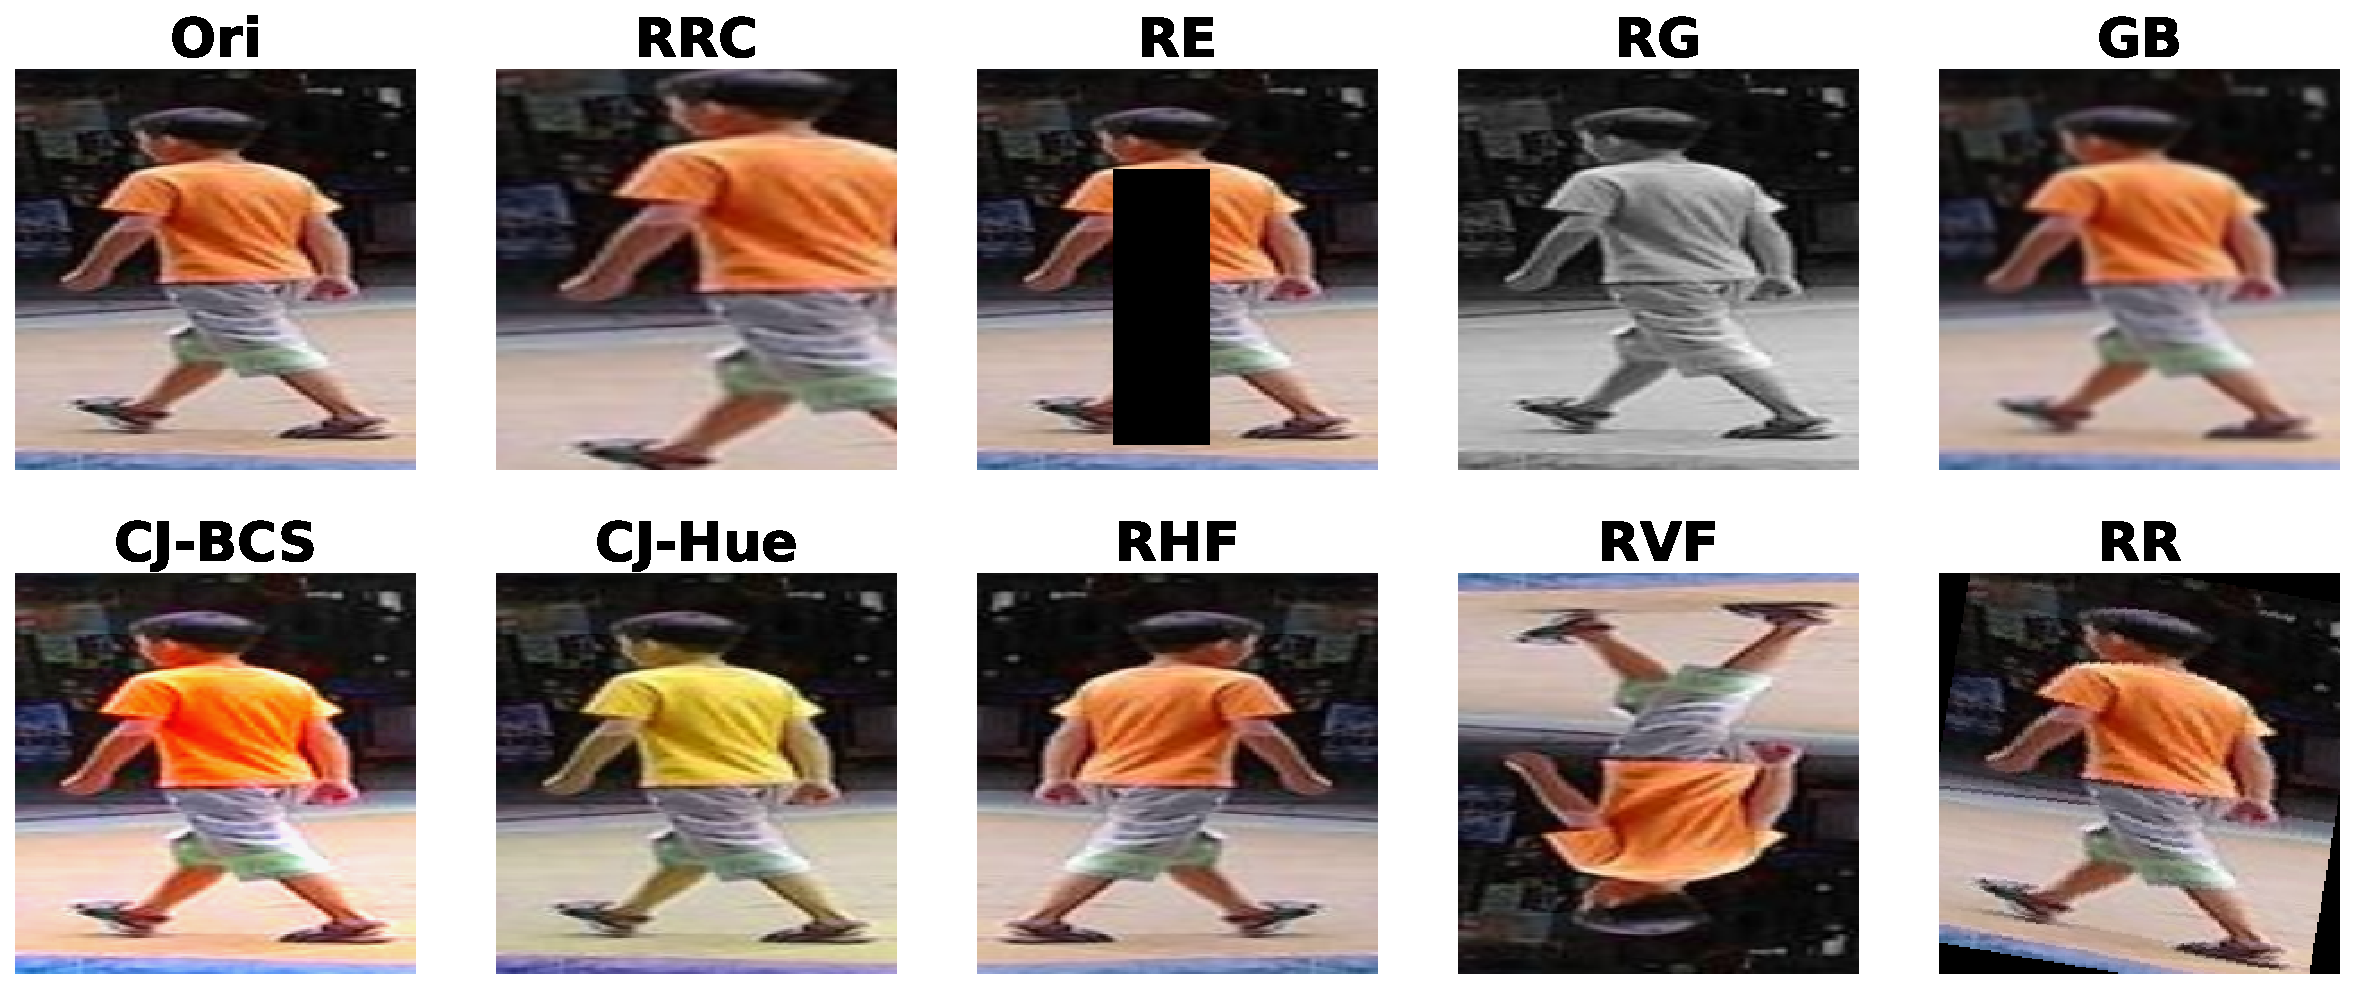
\includegraphics[width=0.98\columnwidth]{figures/figure-aug.pdf}}
% \caption{The original image and the effect of different augmentations. Ori: the original image. RRC: RandomResizedCrop. RE: RandomErasing. RG: RandomGrayscale. GB: GaussianBlur. CJ-BCS: ColorJitter with adjusted brightness, contrast and saturation. CJ-Hue: ColorJitter with adjusted hue. RHF: RandomHorizontalFlip. RVF: RandomVerticalFlip. RR: RandomRotation.} \label{fig:img-aug}
% \end{figure}

We classify image augmentations into two groups: removal and alteration. 
The first group has operations that remove some information from the image, including \emph{RandomResizedCrop}, \emph{RandomErasing}, \emph{RandomGrayscale} and \emph{GaussianBlur}.
The second alters the color or orientation of the image with keeping the main content, including \emph{ColorJitter}, \emph{RandomHorizontalFlip}, \emph{RandomVerticalFlip} and \emph{RandomRotation}.
\emph{These common image augmentations are detailed in the Appendix.}
%The effects of the augmentations, together with hyperparameter descriptions and abaltion study on the hyperparameters are shown in the Appendix.

% Not all image augmentations and their different strengths may be useful. For instance, a moderate magnitude of ColorJitter may improve the model's robustness, while heavy ColorJitter may alter the image too much, making the model challenging to converge. Thus, thorough experiments are conducted to determine which ones and their hyperparameters are effective and can improve the performance of the TBPS task.

% Moreover, several data augmentations may help improve the model's performance, but applying them together on a single image can compromise the performance due to heavy distortion from the original image. Inspired by automatic data augmentation strategies, such as RandAugment~\cite{cubuk2020randaugment} and TrivialAugment~\cite{muller2021trivialaugment}, which apply a fixed number of augmentations randomly, we design an augmentation pool to address this problem. At any given time, only two augmentations from the pool are randomly selected and applied to an image, thus avoiding excessive distortion while still benefiting from a variety of augmentations.

In addition, it should be noted that the simultaneous use of multiple image augmentations may bring heavy distortion to the original image and hurt performance.
Given that, we consider another series of augmentations, they are:
\begin{itemize}
    \item \textit{AutoAugment~\cite{cubuk2018autoaugment}} automatically search for the best augmentation policy, for which reinforcement learning is applied in some augmentation policies. We use its default settings on PyTorch in the experiment.
    %pre-defines some augmentation sub-policies, each containing two operations. A search algorithm is employed to train on a small model and small dataset, in order to decide which sub-policy is most effective at the moment. In this paper, we adopt the best policy for ImageNet, which is the default implementation on PyTorch.
    
    \item \textit{RandAugment~\cite{cubuk2020randaugment}} removes the searching stage in AutoAugment and randomly selects from a pool of augmentation operations. The 2 hyperparameters are the number of augmentations $N$ applied on each image and the magnitude $M$ in the range [1, 31]. We follow the default settings on PyTorch, setting $N$ to 2 and $M$ to 9.
    \item \textit{TrivialAugment~\cite{muller2021trivialaugment}} further drops the requirement of setting hyperparameters in RandAugment, and instead randomly selects one augmentation and its magnitude to apply on each image. Therefore, it is completely parameter-free.
    \item
    \textit{An augmentation pool strategy} is designed in this paper, inspired by the above-mentioned automatic data augmentations. Specifically, two augmentations are randomly selected and applied to each image.
\end{itemize}

%propose an augmentation pool strategy, in which two augmentations are randomly selected and applied to the image, inspired by automatic data augmentation strategies like AutoAugment~\cite{cubuk2018autoaugment}, RandAugment~\cite{cubuk2020randaugment} and TrivialAugment~\cite{muller2021trivialaugment}.

%The simultaneous use of multiple image data augmentations may help to improve the model's performance, on the other hand, could compromise the performance due to heavy distortion from the original image. Given that, we propose an \textbf{Augmentation Pool} containing the effective augmentations, from which two augmentations are randomly selected and applied to an image, inspired by automatic data augmentation strategies like RandAugment~\cite{cubuk2020randaugment} and TrivialAugment~\cite{muller2021trivialaugment}. Thus, excessive distortion is avoided while the model still benefits from the diversity of image augmentations.

% \begin{table}
% \begin{center}
% {\caption{The effects of each text augmentation technique. BT: back translation. SR: synonym replacement. RI: random insertion. RS: random swap. RD: random deletion.}\label{table:txt-aug-demo}}
% \begin{tabular}{c||p{6.0cm}}
% \toprule
% % \rule{0pt}{12pt}
% Method & Sentence \\
% \midrule
% \midrule
% None & a man with short black hair is wearing a white t-shirt, long black pants, red shoes and has a black book\\
% \midrule
% BT & A man with a short black hair is wearing a white T-shirt, long black pants, red shoes, and black books.\\
% \midrule
% SR & a man with \textbf{brusk} black hair is wearing a white t-shirt, long black pants, red shoes and has a black \textbf{playscript}\\
% \midrule
% RI & a man with short black hair is wearing a \textbf{weary} white t-shirt, long black pants, \textbf{fag out} red shoes and has a black book\\
% \midrule
% RS & a \textbf{long} with short black hair is wearing a white t-shirt, \textbf{man} black \textbf{black} red shoes and has a \textbf{pants}, book\\
% \midrule
% RD & a man with short black is wearing a \st{\textbf{white}} t-shirt, long black pants, red shoes and has a black book\\
% \bottomrule
% \end{tabular}
% \end{center}
% \end{table}

\paragraph{Text Augmentation.}
In contrast to image augmentation, there is a smaller pool of available text augmentations due to the abstract and discrete nature of language. 
%We conduct experiments on the following commonly used text augmentation strategies: back translation~\cite{sennrich2015improving}, synonym replacement, random insertion, random swap and random deletion~\cite{wei2019eda}; the effects of them are shown in Table~\ref{table:txt-aug-demo}.

\begin{itemize}
    \item \textit{Back translation} translates the original text to a specific language and then translates it back, by which we can obtain more diverse textual descriptions while preserving its original meaning.
    In our experimental setup, we adopt French as the intermediate language.
    It has a relatively closer form to English and introduces fewer changes to the translated back text in semantics than others.
    
    \item \textit{Synonym replacement} randomly chooses some words from the sentence, and then replaces each of them with a synonym chosen at random.

    \item \textit{Random insertion} randomly chooses some words from the sentence and the synonyms of selected words are then inserted into random positions of the sentence.
    
    \item \textit{Random swap} selects two words from the sentence at random and interchanges their positions. 
    %This process is repeated $n$ times in a sentence.

    \item \textit{Random deletion} randomly removes each word in a sentence.
    %with a probability of $p_{RD}$.

    \item \textit{EDA}~\cite{wei2019eda} randomly selects one from synonym replacement, random insertion, random swap and random deletion and applies it to the sentence.
\end{itemize}

\iffalse
\paragraph{Pair Augmentation.}
Apart from the unimodal augmentations, we explore the augmentation of the image-text pair, inspired by MixGen~\cite{hao2023mixgen}.
Given two image-text pairs $(I_a, T_a)$ and $(I_b, T_b)$, the augmented pair $(I_{aug}, T_{aug})$ is generated by MixGen,
\begin{equation}
% \begin{split}
    I_{aug} = \lambda I_a+(1-\lambda)I_b ~~~~~~
    T_{aug} = \text{concat}(T_a, T_b),
% \end{split}
\end{equation}
where $\lambda$ is a hyperparameter that controls the linear interpolation of raw pixels between $I_a$ and $I_b$. The `$\text{concat}$' directly appends the text $T_b$ after $T_a$.

Following this way for TBPS, the fine-grained semantic information in the original image could be totally broken, and the augmented image does not correspond with the corresponding text.
Alternatively, we propose ConcatGen as: 
\begin{equation}
% \begin{split}
    I_{aug} = \text{concat}(I_a, I_b) ~~~~~~
    T_{aug} = \text{concat}(T_a, T_b),
% \end{split}
\end{equation}
where the `$\text{concat}$' for the image represents the horizontal concatenation of $I_a$ and $I_b$.
\fi
%However, this method shifts the color of the original image and has the fine-grained objects overlapped, as shown in Figure~X, which may have a negative impact on the performance of TBPS task. Intuitively, we propose concatenating the two person images horizontally instead of linearly interpolating them together, named as ConcatGen, thus preserving the original color and all the fine-grained information while generating more data samples at the same time, as shown in Figure~x.

%In both methods, the portion of data samples in each batch replaced with newly generated samples is set to $1/4$ following MixGen.


\subsection{Loss Functions} \label{sec:3.3}

CLIP equips with an image-text contrastive loss to pull positive samples together
while pushing negative ones apart.
% This loss with a minor modification is firstly used in CLIP$^*$.
Further, we normalize the label in the loss and obtain the normalized image-text contrastive loss (N-ITC):
\begin{small}
\begin{equation}
    \mathcal{L}_{N-ITC} = -\frac{1}{2N}( \sum_{i=1}^{N}\sum_{j=1}^{N} \hat{q}_{i,j} \log{p_{i,j}} + \sum_{i=1}^{N}\sum_{j=1}^{N} \hat{q}_{j,i} \log{p_{j,i}}),
    \label{eq:itc}
\end{equation}
\end{small}
where $\hat{q}_{i,j}$ is normalized by ${q_{i,j}}/{\sum_{k=1}^{N} q_{i,k}}$ and $q_{i,j}$ is the ground-truth label ($1$ for positive pair and $0$ for negative one).
$N$ is the number of samples, and 
$p_{i,j}$ represents the pseudo-label that is the probability of matching the image $I_i$ to the text $T_j$ and the reverse applies in $p_{j,i}$,
% \begin{equation} 
%     p_{i,j} = \frac {\exp( f_{I_{i}} \cdot f_{T_{j}} /\tau)}
%         {\sum_{k=1}^{N} \exp( f_{I_{i}} \cdot f_{T_{k}} /\tau)}
%     ~~~~
%     p_{j,i} = \frac {\exp( f_{T_{i}} \cdot f_{I_{j}} /\tau)}
%         {\sum_{k=1}^{N} \exp( f_{T_{i}} \cdot f_{I_{k}} /\tau)},
% \end{equation}
\begin{small}
\begin{equation}
%\begin{aligned}
    p_{i,j} = \frac {\exp( f_{I_{i}} \cdot f_{T_{j}} /\tau)}
        {\sum_{k=1}^{N} \exp( f_{I_{i}} \cdot f_{T_{k}} /\tau)}, 
    p_{j,i} = \frac {\exp( f_{T_{i}} \cdot f_{I_{j}} /\tau)}
        {\sum_{k=1}^{N} \exp( f_{T_{i}} \cdot f_{I_{k}} /\tau)},
%\end{aligned}
\end{equation}
\end{small}
where $f_*$ is the $\ell_2$-normalized representations of the sample, $\tau$ is the learnable temperature parameter.

% Apart from the N-ITC, we study other loss functions under CLIP$^*$ in two directions. 
Apart from the N-ITC, we study other losses in two directions.
One focuses on enhancing data efficiency,
%One focuses on using a limited amount of data to enhance data efficiency, 
and the other targets optimizing the relationship between samples for improving performance.

% Unlike the vanilla contrastive loss with one-hot label, the proposed n-ITC is more effective and robust to TBPS.

% Unlike the vanilla contrastive loss with hard label and only unidirectional image-to-text contrastive learning, the proposed bs-ITC is more effective and robust to TBPS. 

% \begin{equation} 
%     p_{i,j} = \frac {\exp( \left\langle I_{i}, T_{j} \right\rangle/\tau)}
%         {\sum_{k=1}^{N} \exp(sim(I_{i}, T_{k}) /\tau)}
%     ~~
%     p_{j,i} = \frac {\exp(sim(T_{i}, I_{j}) /\tau)}
%         {\sum_{k=1}^{N} \exp(sim(T_{i}, I_{k}) /\tau)},
% \end{equation}
% with $\tau$ being the learnable temperature.

% \begin{equation} \label{eq:label}
%    q_{i,j}^{norm} = \frac{q_{i,j}}{\sum_{k=1}^{N} q_{i,k}}.
% \end{equation}
% The bs-ITC loss is obtained by adjusting the contrastive loss in CLIP.
% The bidirectional soft-contrastive loss is 

% To stabilize the training process, we draw inspiration from ALBEF~\cite{li2021align} and apply the soft label. Specifically, let $q_{i,j}$ denote the one-hot label which equals 1 if samples $i$ and $j$ are a positive pair, otherwise 0; the pseudo-label $q^\prime_{i,j}$ indicates the matching probability between samples $i$ and $j$ inferred by the model. The training label $\mathbf{q}_{i,j}$ is the averaged value of the one-hot label and pseudo-label, formulated as $\mathbf{q}_{i,j} = \frac{1}{2} (q_{i,j} + q^\prime_{i,j})$.

% Beforehand, we apply a bidirectional soft-contrastive loss (bs-ITC) in training model.
% The bs-ITC loss is obtained by adjusting the contrastive loss in CLIP.
% The bidirectional soft-contrastive loss is 
% \begin{equation}
%     \mathcal{L}_{bs-ITC} = \frac{1}{2N}( \sum_{i,j=1}^{N} q_{i,j} \log{p_{i,j}} + \sum_{i,j=1}^{N} q_{j,i} \log{p_{j,i}}),
%     \label{eq:itc}
% \end{equation}
% where $N$ is the number of samples, $q_{i,j}$ and $q_{j,j}$ are the normalization of soft labels described in Section~\ref{sec:3.1}, and $p_{i,j}$ denotes the probabilities of matching $I_i$ to $T_j$, and the reverse applies in $p_{j,i}$, specifically, 
% \begin{equation} 
%     p_{i,j} = \frac {\exp( f^I_{i} \cdot f^T_{j} /\tau)}
%         {\sum_{k=1}^{N} \exp( f^I_{i} \cdot f^T_{j} /\tau)}
%     ~~~~
%     p_{j,i} = \frac {\exp( f^T_{i} \cdot f^I_{j} /\tau)}
%         {\sum_{k=1}^{N} \exp( f^T_{i} \cdot f^I_{j} /\tau)},
% \end{equation}
% with $\tau$ being the learnable temperature.
 
% Unlike the vanilla contrastive loss with hard label and only unidirectional image-to-text contrastive learning, the proposed bs-ITC is more effective and robust to TBPS. 

%we firstly formally describe the contrastive loss in CLIP and introduce our improved contrastive loss for the TBPS-CLIP.

%\paragraph{Normalized Contrastive Loss}
%In original CLIP, The probability of matching ${I_i}$ to ${T_j}$ is defined using softmax function:
%\begin{equation} \label{eq:sim}
%    p_{i,j} = \frac {\exp( h_{I_i} \cdot h_{T_i} /\tau)}
%        {\sum_{j=1}^{N} \exp( h_{I_i} \cdot h_{T_j} /\tau)},
%\end{equation}
%where $h_{I_i}$ and $h_{T_i}$ are the $l^2$-normalized representations of image $I_i$ and text $T_i$, $\tau$ is the learnable temperature.

%CLIP employs cross-entropy loss to pull positive samples together while pushing negative ones apart. For a given batch of images and text, $\{I_{i}\}_{i=1}^{N}$ and $\{T_{j}\}_{j=1}^{N}$, the one-hot label $q_{i,j}$ equals 1 if $i = j$, otherwise 0. The cross-entropy loss from image to text is:
%\begin{equation} \label{eq:i2t}
%    \mathcal{L}_{I2T} = \frac{1}{N} \sum_{i=1}^{N} \sum_{j=1}^{N} \mathbf{q}_{i,j} \log{p_{i,j}},
%\end{equation}
%where $N$ is the batch size, and $\mathbf{q}_{i,j}$ is the soft label of $q_{i,j}$ as described in Section~\ref{sec:3.1}.
% label $q_{i,j} = 1$ if $i = j$, otherwise $q_{i,j} = 0$.
% where $\mathbf{q}_{i,j}$ is the soft label of $q_{i,j}$ introduced in Section~\ref{sec:3.1}.
% In this work, soft label is used as described in Section~\ref{sec:3.1}

%Similarly, the cross-entropy loss from text to image, $\mathcal{L}_{T2I}$, can be formulated by swapping $I$ and $T$ in Equation~\ref{eq:i2t}. Then the overall image-text contrastive loss can be formulated as:
%\begin{equation} \label{eq:itc}
%    \mathcal{L}_{ITC} = \frac{1}{2} (\mathcal{L}_{I2T} + \mathcal{L}_{T2I}).
%\end{equation}

%However, the original contrastive loss in CLIP only sets the one-hot label $y_{i,j}$ to 1 when image $I_i$ and text $T_j$ are a pair, which ignores the identity information. For instance, there may exist text $T_k$ also describing the same identity as $T_j$, but not forming an image-text pair with $I_i$. To address this problem, the positive matches of the same identity are normalized as the label in this work. The normalized label is given by:
%\begin{equation} \label{eq:label}
%    q_{i,j}^{norm} = \frac{q_{i,j}}{\sum_{k=1}^{N} q_{i,k}}.
%\end{equation}

%By replacing the label $\mathbf{q}_{i,j}$ with $\mathbf{q}_{i,j}^{norm}$ in Equation~\ref{eq:i2t}, the normalized contrastive loss $\mathcal{L}_{I2T}^{norm}$ is then formulated as in Equation~\ref{eq:itc}, where $\mathbf{q}_{i,j}^{norm}$ is the soft label of $q_{i,j}^{norm}$ as described in Section~\ref{sec:3.1}

% By applying the training trick described in Section~\ref{sec:3.1}, $\mathbf{q}_{i,j}$

% The normalized contrastive loss from image to text is:
% \begin{equation}
%     \mathcal{L}_{i2t-norm} = \frac{1}{N} \sum_{i=1}^{N} \sum_{j=1}^{N} \mathbf{q}_{i,j} \log{p_{i,j}},
% \end{equation}
% where $\mathbf{q}_{i,j}$ is the soft label of $q_{i,j}$ described in Section~\ref{sec:3.1}.

% After applying the normali

% For both image and text encoders, Transformer encoders are employed. An image $I_i$ of dimensions $H \times W$ is divided into $N$ patches, each of size $P \times P$ pixels. These patches are projected through a shared linear layer into tokens and are preceded by a [CLS] token. The sequence, with a length of $1 + \frac{H \times W}{P^2}$, is then fed into the image encoder. Similarly, a text is tokenized using BPE and concatenated with a [BOS] (beginning of sentence) and an [EOS] (end of sentence) token at the start and end, respectively. The encoded feature corresponding to the [CLS] or [EOS] token is subsequently projected into the same feature space and $l^2$-normalized as the feature vector, denoted as $h_{I_i}$ for images or $h_{T_i}$ for text.

% The probability of matching ${I_i}$ to ${T_j}$ is defined using softmax function:
% \begin{equation} \label{eq:1}
%     p_{i,j} = \frac {\exp( h_{I_i} \cdot h_{T_i} /\tau)}
%         {\sum_{j=1}^{N} \exp( h_{I_i} \cdot h_{T_j} /\tau)}.
% \end{equation}


% To leverage identity information, we normalize the positive matches of the same identity as the label. While the original matching probability of ${I_i}$ and ${T_j}$ is $y_{i,j}$, the normalized one is given by:
% \begin{equation} \label{eq:2}
%     q_{i,j} = \frac{y_{i,j}}{\sum_{k=1}^{N} y_{i,k}},
% \end{equation}
% where $N$ represents the batch size and $\tau$ is a learnable temperature parameter.

% CLIP employs cross-entropy loss to pull positive samples together while pushing negative ones apart. For a given batch of images and text, $\{I_{i}\}_{i=1}^{N}$ and $\{T_{j}\}_{j=1}^{N}$, the cross-entropy loss from image to text is:
% \begin{equation}
%     \mathcal{L}_{i2t-norm} = \frac{1}{N} \sum_{i=1}^{N} \sum_{j=1}^{N} \mathbf{q}_{i,j} \log{p_{i,j}},
% \end{equation}
% where $\mathbf{q}_{i,j}$ is the soft label of $q_{i,j}$ introduced in Section~\ref{sec:3.1}.


% Similarly, the cross-entropy loss from text to image, $\mathcal{L}_{T2I}$, can be formulated by swapping $I$ and $T$ in the equation above. The overall normalized image-text contrastive loss can then be expressed as:
% \begin{equation} \label{eq:4}
%     \mathcal{L}_{itc-norm} = \frac{1}{2} (\mathcal{L}_{I2T} + \mathcal{L}_{T2I}).
% \end{equation}

\subsubsection{Improving Data Efficiency}
\paragraph{Self-Supervision.}
The self-supervised loss (SS) aims at maximizing the similarity between two different augmentations of an image and prompts learning robust feature representations with limited image data.
It has demonstrated effectiveness in various visual tasks~\cite{chen2020simple, chen2021exploring}, and motivates us to explore it in TBPS. 
Specifically, the SS is defined as,
\begin{equation}
\mathcal{L}_{SS} = -\frac{1}{2N} \sum_{i=1}^{2N} \log \frac{\exp(sim(z_i, z_j) / \tau_s)}{\sum_{k=1, k\neq i}^{2N} \exp(sim(z_i, z_k) / \tau_s)},
\end{equation}
where $\tau_s$ is a hyper-parameter and set to $0.1$, and $z_i$ and $z_j$ are the feature representations of two augmentations of the sample. 
The SS can be applied on the image or text or both of them, denoted as SS-I, SS-T and SS-IT, respectively. 

%By applying SS, the model is encouraged to generate consistent feature representations across augmented views and is prompted to learn robust feature representations with limited data.

%Image self-supervised training, which aims at minimizing the distance between two different augmentations of one image, has demonstrated effectiveness in various visual tasks~\cite{he2020momentum, chen2020simple, chen2021exploring}. SLIP~\cite{mu2022slip} applies the image self-supervised training into CLIP for the cross-modal tasks, and has shown significant benefit in data efficiency. It motivates us to explore the self-supervision loss in TBPS task. We apply it to both image and text samples.
% Self-supervised training for images, which minimizes the distance between two different augmentations of a single image, has demonstrated effectiveness in various visual tasks. SLIP~\cite{mu2022slip} applies image self-supervised training within the CLIP framework to pre-train a multi-modal model, and has shown significant improvement in data efficiency.

% Inspired by this, we explore whether fine-tuning the pre-trained CLIP model can benefit from image self-supervision. Furthermore, we investigate whether the same method is applicable to text by maximizing the similarity between two augmentations of the same text.

%Specifically, we borrow SimCLR~\cite{chen2020simple} for the self-supervision loss. It takes two randomly augmented views, $x_i$ and $x_j$, generated from an input sample $x$. Both views are encoded by the encoder and subsequently passed through a projection head, which is a small neural network and maps the feature representation to a lower-dimensional latent space, resulting in $z_i$ and $z_j$. The objective of self-supervision loss is to maximize the similarity between the representations of the two augmented versions of the same sample (\emph{i.e.}, positive pair) while minimizing the similarity with other samples in the batch (\emph{i.e.}, negative pairs). It is achieved using the normalized temperature-scaled cross-entropy loss (NT-Xent loss):
% This is achieved using the normalized temperature-scaled cross-entropy loss (NT-Xent loss):

%The self-supervision loss encourages the model to generate consistent feature representations across augmented views. By introducing this loss into CLIP for TBPS, we take advantage of the unsupervised learning technique to help model learn meaningful feature representations with limited data.

%\begin{figure}
%\centerline{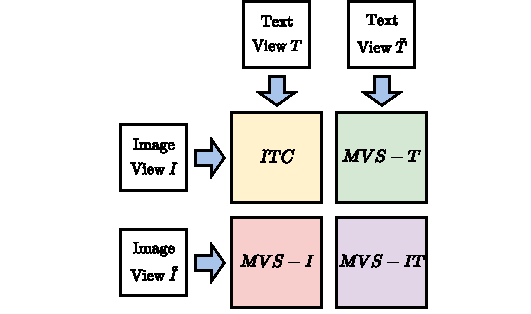
\includegraphics[width=0.5\columnwidth]{figures/fig-mvs.pdf}}
%\caption{Illustration of multi-view supervision.} \label{fig:mvs}
%\end{figure}

\paragraph{Multi-View Supervision.}
%(\emph{i.e.}, a batch of image $I$ and text $T$)
The N-ITC in Equation~\ref{eq:itc} only leverages one augmented view of data. 
Inspired by DeCLIP~\cite{li2021supervision}, more views of samples can provide extra supervision to motivate the potential of limited data.
Specifically, let $\tilde{I}$ and $\tilde{T}$ denote another differently augmented view of $I$ and $T$ by the data augmentation technology, the N-ITC can be applied on ($\tilde{I}, T$) or ($I, \tilde{T}$) or ($\tilde{I}, \tilde{T}$), denoted as the multi-view supervision loss of image (MVS-I), multi-view supervision loss of text (MVS-T), multi-view supervision loss of image and text (MVS-IT), respectively.

%They are denoted as $\mathcal{L}_{MVS-I}$, $\mathcal{L}_{MVS-T}$ and $\mathcal{L}_{MVS-IT}$, respectively. Thus, more additional and diverse high-quality supervision is acquired, as illustrated in Figure~\ref{fig:mvs}. The combination of all additional supervision is denoted as $\mathcal{L}_{MVS-ALL} = \mathcal{L}_{MVS-I} + \mathcal{L}_{MVS-T} + \mathcal{L}_{MVS-IT}$.

% Then the multi-view supervised loss is 
% \begin{equation}
%     \mathcal{L}_{MVS} = \mathcal{L}_{MVS-I} + \mathcal{L}_{MVS-T} + \mathcal{L}_{MVS-IT}.
% \end{equation}

% The multi-view supervised loss results in more additional and diverse high-quality supervision, as illustrated in Figure~\ref{fig:mvs}.

%denoted as $\mathcal{L}_{MVS-I}$, $\mathcal{L}_{MVS-T}$ and $\mathcal{L}_{MVS-IT}$, respectively, resulting in at most 3 more diverse and high-quality additional supervision, as illustrated in Figure~\ref{fig:mvs}. The overall multi-view supervision loss is formulated as:

% DeCLIP~\cite{li2021supervision} adapts the multi-crop transformation from image self-supervised learning~\cite{lecun2021self} to a multimodal setting. Inspired by this, and given that data augmentation strategies in TBPS are systematically studied in this work, we incorporate additional augmented images $I_i^\prime$ and text $T_i^\prime$ as extra supervision. This approach further exploits the potential of the limited data and the data augmentation strategy.

% Specifically, given a matched pair of image $I_i$ and text $T_i$, we can obtain an augmented image $I_i^\prime$ and text $T_i^\prime$. Theoretically, the number of positive pairs has now increased fourfold compared to the original method. These extra samples can be conveniently integrated into the original contrastive loss as described in Equation~\ref{eq:4}.

\subsubsection{Optimization for Retrieval}
% In this section, we present the loss functions employed to optimize our model for the retrieval task.

\paragraph{Reversed Image-Text Contrastive Loss.}

The N-ITC in Equation~\ref{eq:itc} is roughly equivalent to optimizing $D_{\text{KL}}(Q\| P)$, where $Q$ represents the label distribution and $P$ denotes the optimized similarity distribution. 
It mainly focuses on assigning the image-text pair to high similarity probability when its label distribution places high probability (\emph{i.e.}, positive pair).
As a supplement to it, we take inspiration from CMPM~\cite{zhang2018deep} and optimize $D_{\text{KL}}(P\| Q)$, which have $P$ and $Q$ reversed in the N-ITC, and the reversed image-text contrastive loss (R-ITC) considers separating the negative pairs.
% Figure~\ref{fig:kl} vividly presents the difference between the N-ITC and R-ITC. 
Specifically, the R-ITC is formulated as:
% \begin{equation}
% \begin{aligned}
%     \mathcal{L}_{R-ITC} &= \frac{1}{2} (D_{\text{KL}}(p_{i,j} \| \hat{q}_{i,j})+ D_{\text{KL}}(p_{j,i} \| \hat{q}_{j,i})) \\
%     &= \frac{1}{2N} (\sum_{i=1}^{N}\sum_{j=1}^{N} p_{i,j} \log{\frac{p_{i,j}}{\hat{q}_{i,j}+\epsilon}}+ \sum_{i=1}^{N}\sum_{j=1}^{N} p_{j,i} \log{\frac{p_{j,i}}{\hat{q}_{j,i}+\epsilon}}),
% \end{aligned}
% \end{equation}
% \begin{equation}
% \mathsmaller{\begin{aligned}
%     \scalebox{0.8}{$\mathcal{L}_{R-ITC}$} &= \scalebox{0.8}{$\frac{1}{2} (D_{\text{KL}}(p_{i,j} \| \hat{q}_{i,j})+ D_{\text{KL}}(p_{j,i} \| \hat{q}_{j,i}))$} \\
%     &= \scalebox{0.8}{$\frac{1}{2N} (\sum_{i=1}^{N}\sum_{j=1}^{N} p_{i,j} \log{\frac{p_{i,j}}{\hat{q}_{i,j}+\epsilon}}+ \sum_{i=1}^{N}\sum_{j=1}^{N} p_{j,i} \log{\frac{p_{j,i}}{\hat{q}_{j,i}+\epsilon}}),$}
% \end{aligned}}
% \end{equation}
% \begin{equation}
% \mathsmaller{\begin{aligned}
%     \mathcal{L}_{R-ITC} &= \frac{1}{2} (D_{\text{KL}}(p_{i,j} \| \hat{q}_{i,j})+ D_{\text{KL}}(p_{j,i} \| \hat{q}_{j,i})) \\
%     &= \frac{1}{2N} (\sum_{i=1}^{N}\sum_{j=1}^{N} p_{i,j} \log{\frac{p_{i,j}}{\hat{q}_{i,j}+\epsilon}}+ \sum_{i=1}^{N}\sum_{j=1}^{N} p_{j,i} \log{\frac{p_{j,i}}{\hat{q}_{j,i}+\epsilon}}),
% \end{aligned}}
% \end{equation}
\begin{equation}
\resizebox{0.98\columnwidth}{!}{%
$\begin{aligned}
    \mathcal{L}_{R-ITC} &= \frac{1}{2} (D_{\text{KL}}(p_{i,j} \| \hat{q}_{i,j})+ D_{\text{KL}}(p_{j,i} \| \hat{q}_{j,i})) \\
    &= \frac{1}{2N} (\sum_{i=1}^{N}\sum_{j=1}^{N} p_{i,j} \log{\frac{p_{i,j}}{\hat{q}_{i,j}+\epsilon}}+ \sum_{i=1}^{N}\sum_{j=1}^{N} p_{j,i} \log{\frac{p_{j,i}}{\hat{q}_{j,i}+\epsilon}}),
\end{aligned}$%
}
\end{equation}
where $\epsilon$ is a small number to avoid having a zero in the denominator.

% \begin{figure}
% \centerline{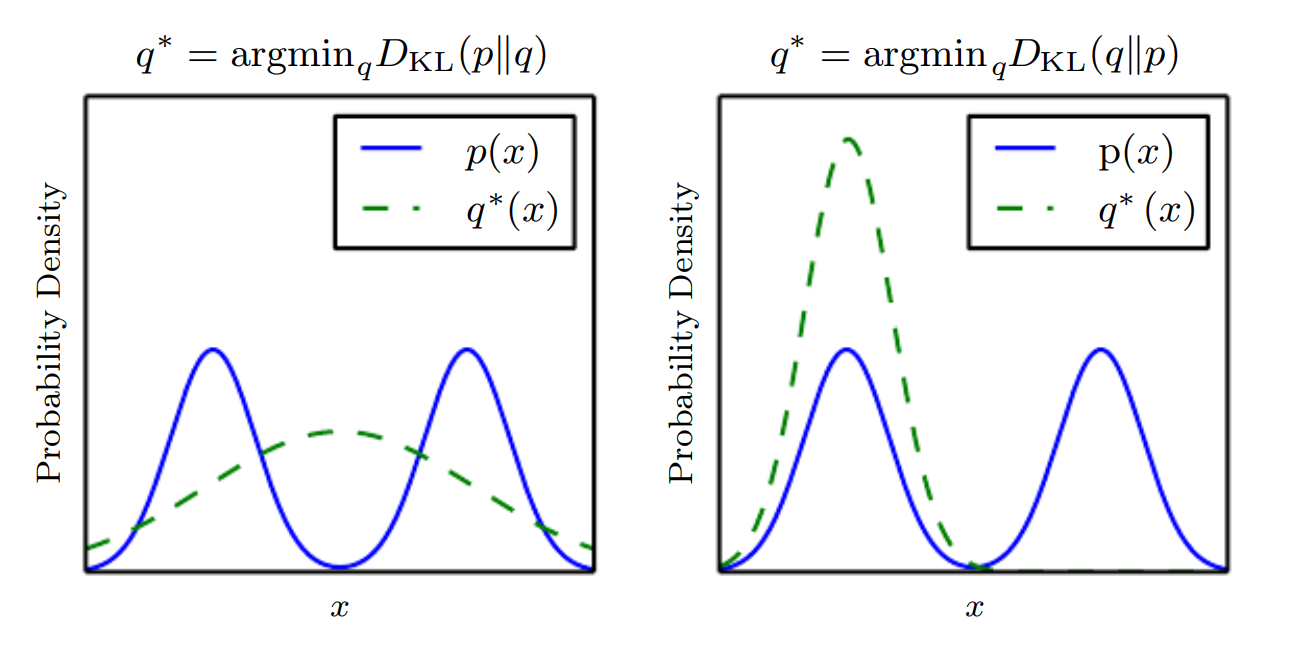
\includegraphics[width=0.98\columnwidth]{figures/dlbook-kl.png}}
% \caption{Illustration of the difference between N-ITC and R-ITC.} \label{fig:kl}
% \end{figure}



%$p$ is the cosine matching probability and $q$ is the normalized label, both of which are the same as those in Equation~\ref{eq:itc}.

% Mathematically, optimizing the image-text contrastive cross-entropy loss $H(Q,P)=H(Q)+D_{\text{KL}}(Q|P)$ is equivalent to optimizing the KL divergence $D_{\text{KL}}(Q|P)$, where $Q$ represents the label and $P$ denotes the similarity distribution to be optimized.

% The cross-modal projection matching (CMPM) loss~\cite{zhang2018deep} is widely used in TBPS methods [xx], and thus also added to the empirical studies.
% It is expressed as:
% \begin{equation}
% \begin{aligned}
%     \mathcal{L}_{CMPM} &= \frac{1}{2} (D_{\text{KL}}(p_{i,j} \| q_{i,j})+ D_{\text{KL}}(p_{j,i} \| q_{j,i})) \\
%     &= \frac{1}{2N} (\sum_{i,j=1}^{N} p_{i,j} \log{\frac{p_{i,j}}{q_{i,j}+\epsilon}}+ \sum_{i,j=1}^{N} p_{j,i} \log{\frac{p_{j,i}}{q_{j,i}+\epsilon}}),
% \end{aligned}
% \end{equation}
% where $\epsilon$ is a small number to avoid having zero in the denominator.

% CMPM minimizes the KL divergence between the projection compatibility distributions $P$ and the normalized matching distributions $Q$, \emph{i.e.}, $D_{\text{KL}}(P\| Q)$.
% As a contrast, the proposed bs-ITC loss in Equation\ref{eq:itc} is similar to optimizing $D_{\text{KL}}(Q\| P)$, which focuses on assigning the image-text pair to high similarity probability when its label distribution places high probability (\emph{i.e.}, positive pair), 
% As a supplement to it, CMPM considers separating the negative pairs.
% Figure~\ref{fig:kl} vividly presents their difference.

%Mathematically, optimizing the image-text contrastive cross-entropy loss $H(Q,P)=H(Q)+D_{\text{KL}}(Q|P)$ is equivalent to optimizing the KL divergence $D_{\text{KL}}(Q|P)$, where $Q$ represents the label and $P$ denotes the similarity distribution to be optimized. This approach mainly focuses on assigning high probability where the label distribution places high probability. However, this can occur even when the label distribution is low, implying that the image-text pair is mismatched, as shown in Figure~\ref{fig:kl}. As a result, negative pairs may not be adequately separated. Our method takes inspiration from CMPM~\cite{zhang2018deep}, which minimizes the KL divergence between the projection compatibility distributions and the normalized matching distributions. Considering the inherent nature of the fine-granular retrieval task, which requires distinguishing between person images with subtle differences, we employ $H(P,Q)$ as supplementary supervision to effectively separate negative pairs.

%Specifically, using $p_{i,j}$ and $q_{i,j}$ as defined in Equations~\ref{eq:sim} and~\ref{eq:label}, the inverse KL divergence from image to text in a batch can be formulated as:

%where $\epsilon$ is a small number to avoid having zero in the denominator. Similarly, the loss $\mathcal{L}_{KL-T2I}$ can be derived from text to image. The inverse KL Divergence loss is defined as:

% \begin{figure}
% \centerline{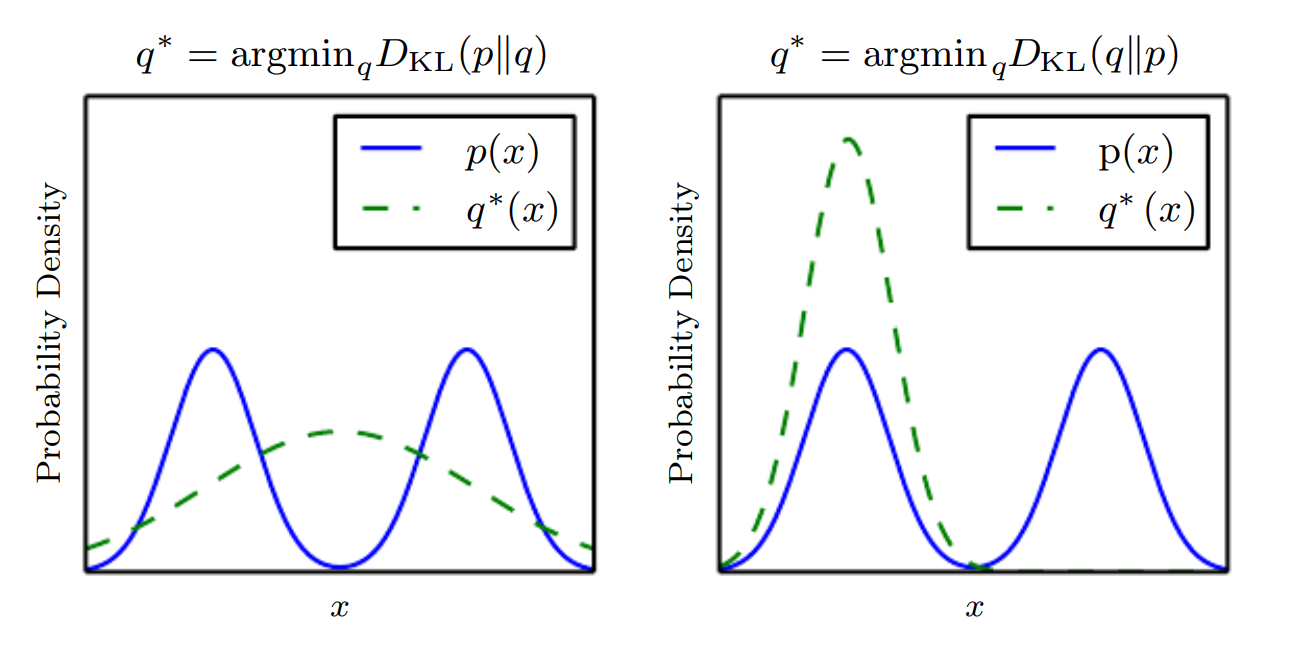
\includegraphics[width=0.98\columnwidth]{figures/dlbook-kl.png}}
% \caption{kl tbd} \label{fig:kl}
% \end{figure}

% The cross-modal projection matching (CMPM) loss~\cite{zhang2018deep} is widely used in TBPS methods [xx], and thus also added to the empirical studies.
% It is expressed as:
% \begin{equation}
% \begin{aligned}
%     \mathcal{L}_{CMPM} &= \frac{1}{2} (D_{\text{KL}}(p_{i,j} \| q_{i,j})+ D_{\text{KL}}(p_{j,i} \| q_{j,i})) \\
%     &= \frac{1}{2N} (\sum_{i,j=1}^{N} p_{i,j} \log{\frac{p_{i,j}}{q_{i,j}+\epsilon}}+ \sum_{i,j=1}^{N} p_{j,i} \log{\frac{p_{j,i}}{q_{j,i}+\epsilon}}),
% \end{aligned}
% \end{equation}
% where $\epsilon$ is a small number to avoid having zero in the denominator.

% CMPM minimizes the KL divergence between the projection compatibility distributions $P$ and the normalized matching distributions $Q$, \emph{i.e.}, $D_{\text{KL}}(P\| Q)$.
% As a contrast, the proposed bs-ITC loss in Equation\ref{eq:itc} is similar to optimizing $D_{\text{KL}}(Q\| P)$, which focuses on assigning the image-text pair to high similarity probability when its label distribution places high probability (\emph{i.e.}, positive pair), 
% As a supplement to it, CMPM considers separating the negative pairs.
% Figure~\ref{fig:kl} vividly presents their difference.

%Mathematically, optimizing the image-text contrastive cross-entropy loss $H(Q,P)=H(Q)+D_{\text{KL}}(Q|P)$ is equivalent to optimizing the KL divergence $D_{\text{KL}}(Q|P)$, where $Q$ represents the label and $P$ denotes the similarity distribution to be optimized. This approach mainly focuses on assigning high probability where the label distribution places high probability. However, this can occur even when the label distribution is low, implying that the image-text pair is mismatched, as shown in Figure~\ref{fig:kl}. As a result, negative pairs may not be adequately separated. Our method takes inspiration from CMPM~\cite{zhang2018deep}, which minimizes the KL divergence between the projection compatibility distributions and the normalized matching distributions. Considering the inherent nature of the fine-granular retrieval task, which requires distinguishing between person images with subtle differences, we employ $H(P,Q)$ as supplementary supervision to effectively separate negative pairs.

%Specifically, using $p_{i,j}$ and $q_{i,j}$ as defined in Equations~\ref{eq:sim} and~\ref{eq:label}, the inverse KL divergence from image to text in a batch can be formulated as:

%where $\epsilon$ is a small number to avoid having zero in the denominator. Similarly, the loss $\mathcal{L}_{KL-T2I}$ can be derived from text to image. The inverse KL Divergence loss is defined as:

\paragraph{Cyclic Image-Text Contrastive Loss.}
The general matching loss (\emph{e.g.}, N-ITC and R-ITC) focuses on optimizing the relationship between the image and text, which may cause the image and text to be irregularly positioned in the representation space, and carries the risk that the query text $T_q$ mistakenly retrieves the negative image $I_n$, while it should match the positive image $I_p$ due to its high similarity with the text $T_p$, as illustrated on the left-hand side of Figure~\ref{fig:cyclip}. 
Following CyCLIP~\cite{goel2022cyclip}, which enhances geometrical consistency in data representation space, we study the cyclic image-text contrastive loss (C-ITC) to mitigate the above problem.
The right-hand side of Figure~\ref{fig:cyclip} shows the geometry of the resulting representation space.

% \begin{figure}
%     \centering
%     \subfloat[Optimizing $\mathcal{L}_{N-ITC}$]{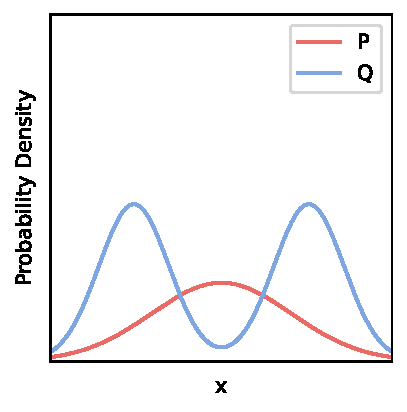
\includegraphics[height=0.35\columnwidth]{figures/fig-kl-qp.pdf}}
%     \hspace{0.03\columnwidth}
%     \subfloat[Optimizing $\mathcal{L}_{R-ITC}$]{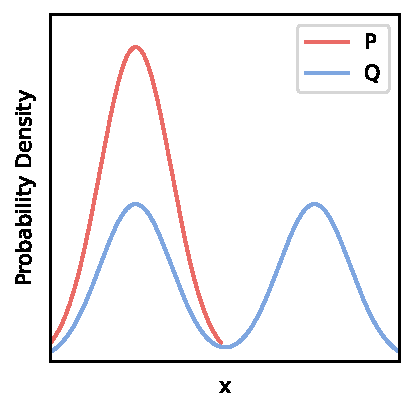
\includegraphics[height=0.35\columnwidth]{figures/fig-kl-pq.pdf}}
%     \caption{Illustration of the difference between N-ITC and R-ITC.}
%     \label{fig:kl}
% \end{figure}
%help improve retrieval performance.

%Illustration of the effect of symmetrization. The left is the original contrastive loss, which only minimizes the distance between a positive pair (\emph{i.e.} ($I_i$, $T_i$) and ($I_j$, $T_j$). Consequently, the given $T_k$, whose semantic is closer to $T_i$, may incorrectly retrieve $I_j$ as $I_j$ is closer to $T_k$ than $I_i$. After applying the symmetrization loss, which impel the red and blue lines of the same color to have the same length, the query $T_k$ correctly matches $I_i$}
\begin{figure}
\setlength{\abovecaptionskip}{0.05cm}
\centerline{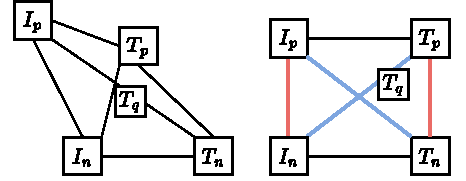
\includegraphics[width=0.75\columnwidth]{figures/fig-cyclip.pdf}}
\caption{Difference between C-ITC (right-hand) and other matching losses (left-hand), \emph{e.g.}, N-ITC and R-ITC. $(I_p, T_p)$ and $(I_n, T_n)$ are two paired cross-modal data and the query text $T_q$ shares the same identity with $(I_p, T_p)$.}
\label{fig:cyclip}
\vspace{-0.5cm}
\end{figure}

Specifically, the learned representations are regularized in two ways: in-modality and cross-modality. 
For the in-modality regularization, the loss enables reducing the gap between the distance of the similarity of two images and that between the corresponding texts:
\begin{equation}
    \mathcal{L}_{C^I-ITC}
    = \frac{1}{N} \sum_{i=1}^N \sum_{j=1}^N (sim(I_i, I_j) - sim(T_i, T_j))^2.
\end{equation}

%: the distance between the first pair's image $I_i$ and the second pair's text $T_j$, and the distance between the second pair's image $I_j$ and the first pair's text $T_i$
For the cross-modality regularization, given two image-text pairs, the gap between their distances is minimized:
\begin{equation}
    \mathcal{L}_{C^C-ITC}
    = \frac{1}{N} \sum_{i=1}^N \sum_{j=1}^N (sim(I_i, T_j) - sim(I_j, T_i))^2.
\end{equation}

Together, the C-ITC can be formulated as:
\begin{equation}
    \mathcal{L}_{C-ITC} = \mathcal{L}_{C^I-ITC} + \mathcal{L}_{C^C-ITC}.
\end{equation}


%where $\lambda$ is set to $0.25$ following CyCLIP~\cite{goel2022cyclip}.

%\subsubsection{Combining the Losses}

%The losses described above are combined using a weighted sum:
%\begin{equation}
%    \mathcal{L} = \lambda_0 (\mathcal{L}_{n-ITC} + \mathcal{L}_{MVS}) + \lambda_1 \mathcal{L}_{SS} + \lambda_2 \mathcal{L}_{rKL} + \lambda_3 \mathcal{L}_{CM},
%\end{equation}
%where the weights $\lambda_0$, $\lambda_1$, $\lambda_2$ and $\lambda_3$ are used to balance the contributions of each loss component in the total loss function. By combining these losses to the modified CLIP, we acquire the complementary strengths of each loss, which ultimately leads to more effective learning and improve TBPS performance.

\subsection{Model Generalization} \label{sec:3.5}
Apart from the empirical study on data augmentation and loss function, 
we also demonstrate the model generalization from two sides.
Specifically, we first apply the proposed TBPS-CLIP to other TBPS methods for verifying the generalization of TBPS-CLIP as the baseline, and then fine-tune TBPS-CLIP based on small amounts of TBPS training data for verifying the generalization of TBPS-CLIP in the few-shot setting. 
We notice that several CLIP variants have been proposed to enhance CLIP's few-shot capability.
Hence, we also conduct the empirical study on two representative few-shot CLIP methods, CoOp~\cite{zhou2022learning} and CLIP-Adapter~\cite{gao2021clip}, for the performance comparison.
\emph{The overview of the two methods is shown in the Appendix.}

% Besides studying the potential of CLIP for TBPS through an empirical study, we make preliminary attempts to examine the few-shot capability of CLIP. For zero-shot learning, we directly apply the off-the-shelf pretrained CLIP to perform TBPS. For few-shot learning,  Specifically, we fine-tune CLIP and the proposed TBPS-CLIP based on small amounts of TBPS training data.  In addition, we notice that several CLIP variants have been proposed to enhance CLIP's few-shot capability. Hence, we conduct the empirical studies on two representative few-shot CLIP methods, CoOp~\cite{zhou2022learning} and CLIP-Adapter~\cite{gao2021clip}. \emph{The overview of the two methods is shown in the Appendix.}


\subsection{Model Compression}  \label{sec:3.4}

%Apart from the empirical studies on augmentation and loss function, 
We provide insight into the model by evaluating the role of each module to the final performance, which is valuable for model compression in real-world applications.
Two evaluation metrics~\cite{wang2020rethinking} are adopted.
The first one evaluates a specific module's contribution by removing the module and observing the performance drop. 
The second one examines the module's importance by measuring how closely the module's weights can approach their initial values while maintaining a certain level of performance. 
\emph{We elaborate on the two metrics in the Appendix.}


\section{Experiments}
The experimental analyses of the empirical studies are detailed in this section. 
Also, although our studies are directed at common technologies to keep the model simple, we provide insights from the TBPS-specific view in this section, \emph{i.e.,} discussing why these technologies can work in TBPS.

Comparisons with other methods are carried out on three benchmark datasets, \emph{i.e.}, CUHK-PEDES~\cite{li2017person}, ICFG-PEDES~\cite{ding2021semantically} and RSTPReid~\cite{zhu2021dssl}, while extensive ablation studies are on the most common CUHK-PEDES.
We use Rank-$k$ and mean Average Precision (mAP) to evaluate the performance.
\emph{The further introduction of dataset, evaluation metric and implementation detail are shown in the Appendix.}

%\textbf{CUHK-PEDES}~\cite{li2017person} is the first TBPS dataset published in $2017$ and the most widely used. This dataset has an average of $3$ images per person, and $2$ textual descriptions accompany each image. It is divided into a training set with $34,054$ images of $11,003$ identities, a validation and a test set containing $3,078$ and $3,074$ images of $1,000$ identities, respectively.

%\textbf{ICFG-PEDES}~\cite{ding2021semantically} is a larger dataset that contains a training set with $34,674$ image-text pairs of $3,102$ identities and a test set with $19,848$ image-text pairs of $1,000$ identities. The images include more complex backgrounds and illumination, and the text description is longer.

%\textbf{RSTPReid}~\cite{zhu2021dssl} is a newly published dataset for suitably handling real scenarios. Each identity has $5$ images captured by different cameras, and each image corresponds to $2$ textual descriptions in this dataset. All are split into three training, validation and test subsets with $3,701$, $200$ and $200$ identities, respectively.



% The loss factors are set as $\{\lambda_0, \lambda_1, \lambda_2, \lambda_3\} = \{1.2, 0.4, 1.0, 1.0\}$; the temperature perameter $\tau_{s}$ in self-supervision loss is set to $0.1$. 
%For self-supervision, the augmentation strategy for image is the same as that in MoCo~\cite{chen2020improved} and SimSiam~\cite{chen2021exploring}, while for text is the same as the most effective combination studied in this work.  
%The random seed is fixed to 1 for reproducibility.


\begin{table}[t]
\setlength{\abovecaptionskip}{-0.01cm}
\begin{center}
{\caption{Ablations of training tricks on CUHK-PEDES. CLIP$^*$ represents CLIP with all four training trick.}\label{table:tricks}}
\resizebox{0.85\columnwidth}{!}{
\begin{tabular}{l!{\vrule}cccc}
\toprule
Methods & Rank-1 & Rank-5 & Rank-10 & mAP   \\
\midrule
% Vanilla CLIP & 60.93 & 81.58 & 88.73 & 54.58 \\ 
CLIP & 60.67 & 81.99 & 88.87 & 54.72 \\ 
CLIP + GlobalGrad & 63.66 &  \textbf{84.08} & 90.11 & 56.46 \\
CLIP + Dropout & 61.06 & 82.00 & 88.95 & 55.10 \\
CLIP + LockBL & 61.27 & 82.23 & 88.79 & 55.43 \\
CLIP + SLabel & 61.53 & 81.99 & 88.71 & 55.22 \\
\midrule
CLIP$^*$ &  \textbf{64.34} & 84.05 &  \textbf{90.51} &  \textbf{57.53} \\
\bottomrule
\end{tabular}
}
\end{center}
\vspace{-0.5cm}
\end{table}

\subsection{Ablations of Training Tricks} \label{sec:4.3}

Starting from CLIP, we first perform experimental investigations on the training tricks discussed in Section~\ref{sec:3.1}. 
As shown in Table~\ref{table:tricks}, all training tricks introduce a positive impact into CLIP on the performance.
%\textbf{By applying the four training tricks together, we obtain CLIP$^*$ with a significant performance improvement of $3.67\%$ at Rank-1 over the vanilla CLIP. It can inspire future works in which the model performance could be boosted through applying these training tricks.}
%We adopt CLIP$^*$ as the baseline in the following ablation experiments.

\subsection{Ablations of Data Augmentation}\label{sec:exp-aug}
%Data augmentation on image, text and image-text pair are ablated in this section. 
%All experiments of data augmentation are based on the CLIP$^*$, with the rank-1 accuracy of 64.34\%.

%\subsubsection{Image Data Augmentation}
We show the optimal results of each augmentation, and analyze their effects.
\emph{The ablation study of the augmentations with different hyperparameters is shown in the Appendix.}

\paragraph{Image Augmentations.} 
Table~\ref{table:image_aug} studies the effect of image augmentations.
(1) In the removal augmentations, RandomResizedCrop and RandomErasing all gain performance enhancement. 
They randomly crop/erase the part of the image, as a result, the augmented image highlights the local details and indirectly encourages the cross-modal fine-grained learning of TBPS.
Unexpectedly, RandomGrayscale, eliminating all colour information from the image, also leads to improved results.
The augmented image without colour by RandomGrayscale is inputted into the model, and the model has to focus on other information (such as texture and shape) during training.
It is well-known that colour information plays a critical role in TBPS~\cite{wu2021lapscore,wang2022caibc}, yet we can learn from the empirical results that other information, except for colour, is also valuable for person retrieval.
In addition, GaussianBlur, smoothing the fine-grained details of the image, significantly impairs performance.
The smoothing operated on the whole image brings the loss of fine-grained information, which is crucial for TBPS.
%(1) In the removal augmentations, RandomResizedCrop and RandomErasing all gain performance enhancement, and even RandomGrayscale, eliminating all color information from the image, also leads to improved results. However, GaussianBlur, smoothing the fine-grained details of the image, significantly impairs performance, probably because these erased details are crucial for TBPS.
(2) In the alternation augmentations, most are beneficial for the performance, including ColorJitter-BCS, RandomHorizontalFlip and RandomRotation. 
They enrich the image diversity without altering the image semantics and strengthen the model's robustness against various images, thus resulting in better performance. By contrast, ColorJitter-Hue and RandomVerticalFlip hurt performance. Both of them change the image semantics. 
The former alters the color, making the color information in the image inconsistent with the corresponding textual description, while the latter dramatically changes the rough shape of the image.
(3) Beyond applying the single augmentation to the image, we conduct experiments of applying multiple augmentations.
Intuitively, we can stack the above effective augmentations to the image (Stacking Together), which leads to performance improvement.
In addition, we can adapt automatic image augmentation strategies AutoAugment~\cite{cubuk2018autoaugment}, RandAugment~\cite{cubuk2020randaugment} and TrivialAugment~\cite{muller2021trivialaugment}.
Nevertheless, the proposed augmentation pool that randomly selects $2$ effective augmentations each time gets the best results.

\begin{table}
\setlength{\abovecaptionskip}{-0.01cm}
\begin{center}
{\caption{Ablations of image augmentations on CUHK-PEDES. `Stacking Together' applies multiple removal and alternation augmentations with the `$\checkmark$' symbol into the image, while `Augmentation Pool' randomly selects two of them in each iteration. `AutoAug', `RandAug' and `TrivialAug' are applied at the default setting.}\label{table:image_aug}}
% \begin{adjustbox}{max width=\textwidth}
\resizebox{0.99\columnwidth}{!}{
\begin{tabular}{l!{\vrule}cccc}
% \hline
\toprule
% \rule{0pt}{12pt}
Methods  & Rank-1 & Rank-5 & Rank-10 & mAP \\
% \hline
\midrule
CLIP$^*$ & 64.34 &  84.05 &  90.51 &  57.53 \\
\midrule
\multicolumn{5}{l}{\textit{The group of removal:}} \\
\midrule
% Baseline & \multicolumn{2}{c}{Modified CLIP} & 64.34 & 84.05 & 57.53 \\
% \midrule
RandomResizedCrop (\checkmark) & 65.29 &  85.01 &  90.68 & 58.62 \\
RandomErasing (\checkmark) & 64.64 &  84.34 &  90.74 &  58.08 \\
RandomGrayscale (\checkmark) &  65.29 &  84.67 &  90.56 & 58.18 \\
GaussianBlur & 55.30 & 77.86 & 85.88 & 49.82 \\
\midrule
\multicolumn{5}{l}{\textit{The group of alternation:}} \\
\midrule
ColorJitter-BCS (\checkmark) &  64.86 &  84.65 &  90.47 &  57.85 \\
ColorJitter-Hue & 64.12 & 84.81 & 90.87 & 57.41 \\
\hdashline[1pt/1pt]
RandomHorizontalFlip (\checkmark) & 65.48 &  84.86 & 90.48 & 58.46 \\
RandomVerticalFlip & 64.23 & 83.98 & 90.16 & 57.35 \\
RandomRotation (\checkmark) &  65.50 &  85.20 &  91.13 &  58.92 \\
\midrule
\multicolumn{5}{l}{\textit{Applying multiple augmentations:}} \\
\midrule
Stacking Together & 65.92 & 85.33 & 90.89 &  59.43 \\
AutoAug~\cite{cubuk2018autoaugment} & 65.43 & 84.84 & 91.07 & 58.55 \\
RandAug~\cite{cubuk2020randaugment} & 65.58 &  \textbf{85.72} & 91.00 & 59.08 \\
TrivialAug~\cite{muller2021trivialaugment} & 65.59 & 84.58 & 90.81 & 58.58 \\
 Augmentation Pool &  \textbf{66.13} & 85.38 &  \textbf{91.21} & \textbf{59.30} \\
\bottomrule
\end{tabular}
}
\end{center}
\vspace{-0.1cm}
\end{table}

%Firstly, augmentations in the group of removal are ablated as shown in the first part of Table~\ref{table:image_aug}. RandomResizedCrop and RandomErasing all gain the performance. Notably, even RandomGrayscale, which eliminates all color information from the image, leads to improved results, highlighting the importance of regularization. However, adjusting blurring the image significantly impairs performance as fine-grained details crucial for TBPS are made indistinguishable.

%Secondly, as displayed in the second part of Table~\ref{table:image_aug}, most data augmentations from the group of alternation are beneficial for the performance, including ColorJitter-BCS, RandomHorizontalFlip and RandomRotation. By contrast, ColorJitter-Hue and RandomVerticalFlip compromise the performance. The former alters the color, making the color information in the image inconsistent with the corresponding caption, while the latter dramatically changes the rough shape of the image.

%Finally, we study applying multiple image augmentations at the same time. Table~\ref{table:image_aug} illustrates that randomly selecting 2 augmentations from a pool each time (\emph{i.e.} Augmentation Pool described in Section~\ref{sec:3.2}), rather than stacking all the augmentations together or using ready-made automatic data augmentation strategies, results in a substantial performance improvement. The rank-1 accuracy has a gain of 1.79\% to achieve 66.13\% by applying image augmentations alone.



% Thus, excessive distortion is avoided while the model still benefits from the diversity of image augmentations.

% Ablation study of each single \textbf{image augmentation} is shown in the upper part of Table~\ref{table:image_aug}, with the effective augmentations highlighted in bold.
% The performance of applying each image augmentation is shown in the top two parts in Table~\ref{table:image_aug}, with the effective ones prepended by checkmarks.
% It is demonstrated that certain image augmentations from both the removal and alternation groups can improve performance. Notably, even RandomGrayscale, which eliminates all color information from the image, leads to improved results, highlighting the importance of regularization. As expected, adjusting the hue or blurring the image significantly impairs performance; the former alters the color information, while the latter diminishes fine-grained details.

% When combining the effective image augmentations, the lower part of Table~\ref{table:image_aug} illustrates that randomly selecting 2 augmentations from a pool each time (\emph{i.e.} Augmentation Pool described in Section~\ref{sec:3.2}), rather than stacking all the augmentations together or using ready-made automatic data augmentation strategies like RandAugment, results in a substantial performance improvement. The rank-1 accuracy has a gain of 1.79\% to achieve 66.13\% by applying image augmentations alone.


\begin{table}[t]
\setlength{\abovecaptionskip}{-0.01cm}
\begin{center}
{\caption{Ablations of text augmentations on CUHK-PEDES. `Stacking Together' applies multiple augmentations with the `$\checkmark$' symbol into the text.}\label{table:text_aug}}
% SR: synonym replacement. RI: random insertion. RS: random swap. RD: random deletion.
\resizebox{0.95\columnwidth}{!}{
\begin{tabular}{l!{\vrule}cccc}
\toprule
% \rule{0pt}{12pt}
Methods & Rank-1 & Rank-5 & Rank-10 & mAP \\
\midrule
CLIP$^*$ & 64.34 &  84.05 &  90.51 &  57.53 \\
\midrule
Back Translation (\checkmark) & 64.77 &  \textbf{84.67} &  90.56 &  57.49 \\
Synonym Replacement & 63.95 & 83.76 & 89.96 & 56.90 \\
Random Insertion & 63.71 & 84.29 & 90.03 & 56.77 \\
Random Swap & 56.41 & 79.08 & 86.14 & 49.29 \\
Random Deletion (\checkmark) &  65.53 &  84.70 &  \textbf{90.87} &  57.90 \\
EDA~\cite{wei2019eda} & 63.43 & 83.77 & 90.27 & 56.15 \\
\midrule
 Stacking Together &  \textbf{65.72} & 84.62 &  90.76 & \textbf{58.68} \\
\bottomrule
% \multicolumn{6}{c}{\multirow{2}{*}{\shortstack{SR: synonym replacement. RI: random insertion. \\RS: random swap. RD: random deletion.}}}
\end{tabular}
}
\end{center}
\vspace{-0.5cm}
\end{table}

\begin{table}[t]
\setlength{\abovecaptionskip}{-0.01cm}
\begin{center}
{\caption{Results of combining optimal augmentations within each modality.}\label{table:aug_all}}
\resizebox{0.93\columnwidth}{!}{
\begin{tabular}{l!{\vrule}cccc}
\toprule
% \rule{0pt}{12pt}
Methods & Rank-1 & Rank-5 & Rank-10 & mAP \\
\midrule
 CLIP$^*$ &  64.34 &   84.05 &  90.51 &  57.53 \\
\midrule
Image Aug & 66.13 & 85.38 & 91.21 & 59.30 \\
Text Aug & 65.72 & 84.62 & 90.76 & 58.68 \\
  Image \& Text Aug &  \textbf{66.78} &  \textbf{85.98} &  \textbf{91.23} &  \textbf{59.68} \\
\bottomrule
\end{tabular}
}
\end{center}
\vspace{-0.1cm}
\end{table}

\begin{table}[t]
\setlength{\abovecaptionskip}{-0.01cm}
\begin{center}
{\caption{Ablations of loss functions on CUHK-PEDES. `Stacking Together' denotes that multiple losses with the `$\checkmark$' symbol are used to CLIP$^*$+Aug .}\label{table:loss}}
% \begin{adjustbox}{max width=\textwidth}
\resizebox{0.48\textwidth}{!}{
\begin{tabular}{l!{\vrule}cccc}
% \hline
\toprule
% \rule{0pt}{12pt}
Methods & Rank-1 & Rank-5 & Rank-10 & mAP \\
% \hline
\midrule
CLIP$^*$+Aug & 66.78 & 85.98 & 91.23 & 59.68 \\
\midrule
N-ITC (\checkmark) & 66.91 & 85.98 & 91.68 & 60.01 \\
\midrule
\multicolumn{5}{l}{\textit{Improving data efficiency:}} \\
\midrule
% Baseline & \multicolumn{2}{c}{Modified CLIP} & 64.34 & 84.05 & 57.53 \\
% \midrule
SS-I (\checkmark) & 67.54 & 86.13 &  \textbf{91.78} & 60.94 \\
SS-T & 65.97 & 85.40 & 90.72 & 59.10 \\
SS-IT & 66.81 & 86.09 & 91.63 & 59.82 \\
\hdashline[1pt/1pt]
MVS-I (\checkmark)\rule{0pt}{8pt} & 67.50 & 86.45 & 91.63 & 60.84 \\
MVS-T & 66.46 & 85.96 & 91.13 & 60.24 \\
MVS-IT & 67.01 & 85.66 & 91.33 & 59.83 \\
\midrule
\multicolumn{5}{l}{\textit{Optimization for retrieval:}} \\
\midrule
R-ITC (\checkmark) &  68.19 & 86.01 & 90.94 & 60.90 \\
C-ITC (\checkmark) & 67.15 & 86.31 & 92.04 & 60.58 \\
\midrule
\multicolumn{5}{l}{\textit{Applying multiple losses:}} \\
\midrule
 Stacking Together (TBPS-CLIP) &  \textbf{69.54} &  \textbf{86.99} & 91.24 &  \textbf{61.57} \\
\bottomrule
\end{tabular}
}
\end{center}
\vspace{-0.5cm}
\end{table}


\paragraph{Text Augmentations.} 
As presented in Table~\ref{table:text_aug}, the effective text augmentations for TBPS are the back translation and random deletion.
The back translation directly enriches the forms of the original texts, and the random deletion plays a role of regularization by randomly dropping some words,
both of which positively impact performance.
Accordingly, applying the two together (Stacking Together) leads to an improvement of $1.38\%$ at Rank-1.
On the contrary, the synonym replacement, random insertion and random swap all hurt performance by a margin.
They come with risks of distorting the text's original meaning, and specifically, the random insertion and random swap tend to break the original structure of the sentence.
These make the text encoder harder to comprehend the augmented text.
Consequently, it is reasonable that EDA, selecting one among these at random, does not bring performance enhancement.

%As of text augmentation, the effective ones are random deletion and back translation, as shown in Table~\ref{table:text_aug}. Random deletion plays a role of regularization by randomly dropping non-stop words with a fixed probability, while back translation directly enrich the forms of original texts. Applying the two together leads to an improvement of 1.38\%, reaching 65.72\% rank-1 accuracy.

%However, synonym replacement, random insertion and random swap all compromise the performance by a margin, as synonym replacement and random insertion may introduce some words that are not exact synonyms of the original words, distorting the original meaning of the sentence, as shown in the Appendix; random insertion and random swap break the original structure of the sentence, making the text encoder harder to comprehend the original meaning.

%\paragraph{Pair Augmentation.} 
%According to the results in Table~\ref{table:pair_aug}, directly applying MixGen~\cite{hao2023mixgen} to the image-text pair shows suboptimal performance, as the content of two images is linearly mixed, making it hard to distinguish fine-grained details from others. Applying the proposed ConcatGen alleviates this issue and reaches a higher performance than MixGen, yet still lags behind CLIP$^*$. The concatenation of images in ConcatGen significantly changes the original layout of the image, and the images with different layouts inputted to the model could perturb the training process.

\iffalse
\begin{table}
\begin{center}
{\caption{Ablations of image-text pair augmentations on CUHK-PEDES.}\label{table:pair_aug}}
\resizebox{1\columnwidth}{!}{
\begin{tabular}{l!{\vrule}cccc}
\toprule
% \rule{0pt}{12pt}
Methods & Rank-1 & Rank-5 & Rank-10 & mAP \\
\midrule
CLIP$^*$ &   \textbf{64.34} & 84.05 &  \textbf{90.51} &  \textbf{57.53} \\
\midrule
MixGen~\cite{hao2023mixgen} & 63.87 &  \textbf{84.26} & 90.03 & 57.16 \\
ConcatGen & 64.13 & 83.29 & 89.80 & 57.08 \\
\bottomrule
\end{tabular}
}
\end{center}
\end{table}
\fi

%When applying \textbf{image-text pair augmentation}, according to Table~\ref{table:pair_aug}, directly utilizing MixGen shows suboptimal performance, as the content of two image samples are linearly mixed together, making it hard to distinguish fine-grained details. Applying our proposed ConcatGen alleviates this issue and reaches a performance higher than MixGen, but still lags behind the baseline. This may due to the changes in areas of concern in the image. Specifically, the area of certain parts of a person is relatively fixed in the image. However, after two person images are concatenated horizontally, the positions of details (\emph{i.e.} appearance, clothing, etc.) where the model should pay attention to is changed, thus perturbing the training process.


\paragraph{Together with Optimal Augmentations.}
As shown in Table~\ref{table:aug_all}, based on the CLIP$^*$, after combining all optimal data augmentations (\emph{i.e.}, `Augmentation Pool' for image, `Stacking Together' for text), the Rank-1 accuracy is significantly increased by $2.44\%$.
It is worth stressing that the gain is only from exploiting data augmentations.

\subsection{Ablations of Loss Functions}
Table~\ref{table:loss} studies the effectiveness of the loss functions.
(1) Compared to CLIP$^*$+Aug in which the original image-text contrastive loss is used, replacing the loss with the normalized image-text contrastive loss (N-ITC) brings a slight improvement of $0.13\%$ at Rank-1.
(2) For the loss functions that aim to improve data efficiency, it is shown that the image self-supervision (SS-I) achieves the best performance among SS-I, SS-T and SS-IT, and similarly, the multi-view supervision of image (MVS-I) gets the best within MVS-I, MVS-T and MVS-IT. These indicate that improving data efficiency by exploiting image data is more effective than text data in TBPS.
(3) For the loss functions that are optimized for retrieval, both R-ITC and C-ITC improve the performance. In particular, R-ITC leads to a significant boost of $1.41\%$ than CLIP+Aug, showing the significance of R-ITC with the constraint of pulling negative samples apart.
Finally, we combine all of these effective losses, boosting performance by a large margin of $2.76\%$ at Rank-1 based on CLIP$^*$+Aug, achieving $69.54\%$ Rank-1 accuracy.

%The effectiveness of these losses have been verified in various common cross-modal tasks~\cite{chen2020simple, chen2021exploring,li2021supervision,goel2022cyclip}. Correspondingly, as the above experimental results show, they can also be effectively applied in TBPS (a human-centric cross-modal task). It is not just that a customized task-oriented loss only works in TBPS.

%In this section, ablation study on the loss functions are carried out, as listed in Table~\ref{table:loss}; the baseline is CLIP$^*$ with the final data augmentation strategy studied in Section~\ref{sec:exp-aug}.

%Firstly, normalized label slightly helps improves the original contrastive loss, resulting in a performance gain of $0.13\%$.

%Secondly, the loss functions to improve data efficiency are ablated. As can be seen in Table~\ref{table:loss}, for self-supervision loss, image self-supervision boosts the performance while text self-supervision does not; Applying self-supervision of image only also shows an advantage over that of both image and text. As of multi-view supervision loss, adding an additional image view as a supervision improves the performance, while adding additional text view does not. Multi-view supervision using both addition image and text does not show as much performance gain as using image alone. These indicate that utilizing text information may not be straightforward as image, and may need a different approach; this accords with our data augmentation experiment that augmenting text does not have as much performance boost as image, and there are fewer effective ways to implement text augmentation. In general, improving data efficiency by exploiting image data is demonstrated to be effective.

%Thirdly, the two loss functions to optimize for retrieval are studied. CMPM and cyclic matching loss all improve the performance. It is worth noting that CMPM loss leads to a significant boost of $1.41\%$, showing the significance of pulling negative samples apart.

%Finally, the effective losses with check marks prepended in Table~\ref{table:loss} are combined. This makes the performance increase from the baseline by a large margin of $2.76\%$, achieving $69.54\%$ rank-1 accuracy.

% Table~\ref{table:loss} demonstrates that implementing the loss functions mentioned in Section~\ref{sec:3.3} individually contributes to improved performance. Consequently, the final performance significantly exceeds that of using the original image-text contrastive loss alone.

% The effectiveness of implementing each loss alongside the original contrastive loss in CLIP is first studied, based on the modified CLIP with data augmentation implemented. After that, the effective ones are then combined together to obtain the best performance.

% As can be seen in Table~\ref{table:loss}, using normalized contrastive loss and implementing the four proposed losses in Section~\ref{sec:loss} all achieve a performance gain over the original contrastive loss. More specifically, image self-supervision boosts the performance while text self-supervision does not. Also, in multi-view supervision, adding an additional image view as a supervision improves the performance, while adding additional text view does not. These indicate that utilizing text information may not be straightforward as image, and may need a different approach; this accords with our data augmentation experiment that augmenting text does not have as much performance boost as image, and there are fewer effective ways to implement text augmentation.

% As a result, image self-augmentation is adopted as the only self-supervision loss, such that $\mathcal{L}_{SS} = \mathcal{L}_{SS-I}$, and additional image view is leveraged to implement the multi-view supervision, such that $\mathcal{L}_{MVS} = \mathcal{L}_{MVS-I}$. Applying the effective losses one by one leads to a steady rise of performance, as listed in Table~\ref{table:loss}. Consequently, applying all the effective losses leads to a performance rise of 2.76\%, achieving a rank-1 accuracy of 69.54\%.

%GNA-RNN~\cite{li2017person} & 19.05 & - & 53.64 & - \\ 
%TIPCB~\cite{chen2022tipcb} &Neurocomputing22& 63.63 & 82.82 & 89.01 & - \\
\begin{table}[t]
\setlength{\abovecaptionskip}{-0.01cm}
\begin{center}
{\caption{Comparisons with state-of-the-art methods on CUHK-PEDES.}\label{table:cmp_cuhk}}
\resizebox{0.49\textwidth}{!}{
\begin{tabular}{l!{\vrule}l!{\vrule}cccc}
\toprule
% \rule{0pt}{12pt}
Methods & References & Rank-1 & Rank-5 & Rank-10 & mAP   \\
\midrule
\multicolumn{6}{l}{\textit{w/o CLIP:}} \\
\midrule
%CMPM/C~\cite{zhang2018deep} &ECCV18& 49.37 & - & 79.27 & - \\ 
% TIMAM~\cite{sarafianos2019adversarial} &ICCV19& 54.51 & 77.56 & 84.78 & - \\
ViTAA~\cite{wang2020vitaa} &ECCV20& 55.97 & 75.84 & 83.52 & - \\
DSSL~\cite{zhu2021dssl} &MM21& 59.98 & 80.41 & 87.56 & - \\
SSAN~\cite{ding2021semantically} &arXiv21& 61.37 & 80.15 & 86.73 & - \\
LapsCore~\cite{wu2021lapscore} &ICCV21& 63.40 & - & 87.80 & - \\
CAIBC~\cite{wang2022caibc} &MM22& 64.43 & 82.87 & 88.37 & - \\
LGUR~\cite{shao2022learning} &MM22& 65.25 & 83.12 & 89.00 & - \\
AXM-Net~\cite{farooq2022axm} &AAAI22& 64.44 & 80.52 & 86.77 & 58.73 \\
IVT~\cite{shu2023see} &ECCVW22& 65.59 & 83.11 & 89.21 & 60.66 \\
SAF~\cite{li2022learning} &ICASSP22& 64.13 & 82.62 & 88.40 & 58.61 \\
RaSa~\cite{bai2023rasa} &IJCAI23&   \textbf{76.51} &   \textbf{90.29} &   \textbf{94.25} &   \textbf{69.38} \\
\midrule
\multicolumn{6}{l}{\textit{w/ CLIP:}} \\
\midrule
TBPS-LD~\cite{han2021text} &BMVC21& 64.08 & 81.73 & 88.19 & 60.08 \\
CFine~\cite{yan2022clip} &arXiv22& 69.57 & 85.93 & 91.15 & - \\
TP-TPS~\cite{wang2023exploiting} &arXiv23& 70.16 & 86.10 & 90.98 &   66.32 \\
IRRA (ViT-B/16)~\cite{jiang2023cross} &CVPR23& 73.38 &   \textbf{89.93} &   \textbf{93.71} & \textbf{66.13} \\
% \hline
\midrule
CLIP (ViT-B/32) &Baseline& 60.67 & 81.99 & 88.87 & 54.72 \\
TBPS-CLIP (ViT-B/32) &Ours& 69.54 & 86.99 & 91.24 & 61.57 \\
CLIP (ViT-B/16) &Baseline& 65.37 & 85.83 & 91.59 & 59.42 \\
  TBPS-CLIP (ViT-B/16) &Ours&   \textbf{73.54} & 88.19 & 92.35 & 65.38 \\
\hdashline
Simplified TBPS-CLIP (ViT-B/16) &Ours& 72.66 & 88.14 & 92.72 & 64.97 \\
\bottomrule
\end{tabular}
}
\end{center}
\vspace{-0.1cm}
\end{table}

%TIPCB~\cite{chen2022tipcb} &Neuro22& 54.96 & 74.72 & 81.89 & - \\
\begin{table}
\setlength{\abovecaptionskip}{-0.01cm}
\begin{center}
\caption{Comparisons with state-of-the-art methods on ICFG-PEDES.}\label{table:cmp_icfg}
\resizebox{0.49\textwidth}{!}{
\begin{tabular}{l!{\vrule}l!{\vrule}cccc}
\toprule
Methods & References & Rank-1 & Rank-5 & Rank-10 & mAP   \\
\midrule
\multicolumn{6}{l}{\textit{w/o CLIP:}} \\
\midrule
%CMPM/C~\cite{zhang2018deep} &ECCV18& 43.51 & 65.44 & 74.26 & - \\
ViTAA~\cite{wang2020vitaa} &ECCV20& 50.98 & 68.79 & 75.78 & - \\
SSAN~\cite{ding2021semantically} &arXiv21& 54.23 & 72.63 & 79.53 & - \\
LGUR~\cite{shao2022learning} &MM22& 57.42 & 74.97 & 81.45 & - \\
IVT~\cite{shu2023see} &ECCVW22& 56.04 & 73.60 & 80.22 & - \\
SAF~\cite{li2022learning} &ICASSP22& 54.86 & 72.13 & 79.13 & 32.76 \\
RaSa~\cite{bai2023rasa} &IJCAI23&   \textbf{65.28} &   \textbf{80.40} &   \textbf{85.12} &   \textbf{41.29} \\
\midrule
\multicolumn{6}{l}{\textit{w/ CLIP:}} \\
\midrule
TP-TPS~\cite{wang2023exploiting} &arXiv23& 60.64 & 75.97 & 81.76 &  \textbf{42.78} \\
CFine~\cite{yan2022clip} &arXiv22& 60.83 & 76.55 & 82.42 & - \\
IRRA (ViT-B/16)~\cite{jiang2023cross} &CVPR23& 63.46 & 80.25 &  \textbf{85.82} & 38.06 \\
\midrule
CLIP (ViT-B/32) &Baseline& 53.96 & 73.69 & 80.43 & 32.37 \\
TBPS-CLIP (ViT-B/32) &Ours& 59.88 & 77.40 & 83.33 & 34.96  \\
CLIP (ViT-B/16) &Baseline& 55.97 & 74.62 & 81.35 & 30.63 \\
  TBPS-CLIP (ViT-B/16) &Ours&   \textbf{65.05} &   \textbf{80.34} & 85.47 & 39.83 \\
\hdashline
Simplified TBPS-CLIP (ViT-B/16) &Ours& 64.52 & 80.03 & 85.39 & 39.54
 \\
\bottomrule
\end{tabular}
}
\end{center}
\vspace{-0.5cm}
\end{table}

\begin{table}[t]
\setlength{\abovecaptionskip}{-0.01cm}
\begin{center}
{\caption{Comparisons with state-of-the-art methods on RSTPReid.}\label{table:cmp_rstp}}
\resizebox{0.49\textwidth}{!}{
\begin{tabular}{l!{\vrule}l!{\vrule}cccc}
\toprule
Methods & References & Rank-1 & Rank-5 & Rank-10 & mAP \\
\midrule
\multicolumn{6}{l}{\textit{w/o CLIP:}} \\
\midrule
DSSL~\cite{zhu2021dssl} &MM21& 39.05 & 62.60 & 73.95 & - \\
SSAN~\cite{ding2021semantically} &arXiv21& 43.50 & 67.80 & 77.15 & - \\
IVT~\cite{shu2023see} &ECCVW22& 46.70 & 70.00 & 78.80 & - \\
SAF~\cite{li2022learning} &ICASSP22 & 44.05 & 67.30 & 76.25 & 36.81 \\
RaSa~\cite{bai2023rasa} &IJCAI23&   \textbf{66.90} &   \textbf{86.50} &   \textbf{91.35} &   \textbf{52.31} \\
\midrule
\multicolumn{6}{l}{\textit{w/ CLIP:}} \\
\midrule
CFine~\cite{yan2022clip} &arXiv22& 50.55 & 72.50 & 81.60 & - \\
TP-TPS~\cite{wang2023exploiting} &arXiv23& 50.65 & 72.45 & 81.20 & 43.11 \\
IRRA (ViT-B/16)~\cite{jiang2023cross} &CVPR23& 60.20 & 81.30 & 88.20 & 47.17 \\
\midrule
% Baseline (ViT-B/32) & 48.65 & 72.75 & 81.65 & 38.33 \\ 2
% Ours (ViT-B/32) & 55.00 & 78.30 & 86.65 & 43.11 \\ 2
CLIP (ViT-B/32) &Baseline& 50.10 & 76.10 & 84.95 & 41.14 \\
TBPS-CLIP (ViT-B/32) &Ours& 56.65 & 80.75 & 87.30 & 44.00 \\
CLIP (ViT-B/16) &Baseline& 56.15 & 78.30 & 86.60 & 43.26 \\
TBPS-CLIP (ViT-B/16) &Ours& 61.95 &   \textbf{83.55} &   \textbf{88.75} &   \textbf{48.26} \\
\hdashline
  Simplified TBPS-CLIP (ViT-B/16) &Ours&   \textbf{62.10} & 81.90 & 87.75 & 48.00
 \\
\bottomrule
\end{tabular}
}
\end{center}
\vspace{-0.1cm}
\end{table}

\subsection{Comparisons with State-of-the-Art Methods} 
We compare TBPS-CLIP with state-of-the-art methods
on CUHK-PEDES, ICFG-PEDES and RSTPReid datasets, as shown in Table~\ref{table:cmp_cuhk}, Table~\ref{table:cmp_icfg} and Table~\ref{table:cmp_rstp}, respectively.

(1) In comparison with the methods using CLIP, the proposed TBPS-CLIP with ViT-B/16 as the image encoder outperforms the state-of-the-art method IRRA by a margin on ICFG-PEDES and RSTPReid, and performs on par with it on CUHK-PEDES.
It is worth noting that IRRA appends a multimodal interaction encoder after CLIP for obtaining superior performance, while the proposed TBPS-CLIP keeps it simple in the network architecture (\emph{i.e.,} original two-stream network architecture of CLIP) and also achieves promising results.
\textbf{It can be clearly seen from Table~\ref{table:cmp_sota} that TBPS-CLIP is more lightweight than IRRA.
TBPS-CLIP prompts CLIP to utilize and mine data efficiently, enabling the network to be trained merely with 5 epochs. 
The highly efficient training makes it very friendly as a baseline.}
(2) In comparison with the methods without CLIP, we notice that RaSa performs strongly.
It adopts ALBEF~\cite{li2021align} as the baseline and contains two models, an online model and its momentum version, each consisting of an image encoder, a text encoder and a cross-modal encoder.
\textbf{Although having outstanding performance, RaSa is cumbersome and challenging to support its generalization, as shown in Table~\ref{table:cmp_sota}.
The proposed TBPS-CLIP, with very lightweight and low-cost architecture and promising performance, has the potential as a baseline to provide broader applications.}
(3) Considering the convenience of applying TBPS-CLIP as the baseline, we further provide a simplified TBPS-CLIP, in which there are only N-ITC and R-ITC losses. It still performs satisfactorily, specifically, even beats IRRA on ICFG-PEDES and RSTPReid.
The simplified TBPS-CLIP equipped with two losses can be more easily applied as a baseline in further work.

\begin{table}[t]
\setlength{\abovecaptionskip}{-0.01cm}
\begin{center}
{\caption{Comparisons with recently SOTA methods on CUHK-PEDES. Param.(M) and Epoch denote the number of modal parameters  (in millions) and the number of epochs in training, respectively. Time(s) represents the online running time (in seconds).}\label{table:cmp_sota}}
\resizebox{0.49\textwidth}{!}{
\begin{tabular}{l!{\vrule}l!{\vrule}cccc}
\toprule
\multirow{2}{*}{Methods} & \multirow{2}{*}{Baselines} & \multirow{2}{*}{Param.(M)} & \multirow{2}{*}{Epoch} & \multicolumn{2}{c}{Time(s)} \\
&  &  &  & Training & Test \\
\midrule
RaSa~\cite{bai2023rasa} & ALBEF & 210.2 & 30 & 27967.5 & 869.8 \\
IRRA~\cite{jiang2023cross} & CLIP (ViT-B/16) & 194.5 & 60 & 6110.4 & 31.4 \\
TBPS-CLIP (Ours) & CLIP (ViT-B/16) & 149.2 & 5 & 1234.7 & 31.4 \\
\bottomrule
\end{tabular}
}
\end{center}
\vspace{-0.5cm}
\end{table}

\begin{table}[t]
\setlength{\abovecaptionskip}{-0.01cm}
\begin{center}
{\caption{Results for applying the proposed TBPS-CLIP as the baseline of other method on CUHK-PEDES. The mean Inverse Negative Penalty(mINP) metric is used in IRRA and also adopted here for comparison.}\label{table:genera}}
\resizebox{0.49\textwidth}{!}{
\begin{tabular}{l!{\vrule}l!{\vrule}ccccc}
\toprule
Methods & Baselines & Rank-1 & Rank-5 & Rank-10 & mAP & mINP \\
\midrule
IRRA & CLIP & 73.38 & 89.93 & 93.71 & 66.13 & 50.24 \\
\hdashline
IRRA$^*$ & TBPS-CLIP & 74.97 & 89.82 & 93.80 & 67.84 & 52.53 \\
IRRA$^*$ & Simplified TBPS-CLIP & 74.56	& 89.26	& 93.52	& 67.52 & 52.58 \\
\bottomrule
\end{tabular}
}
\end{center}
\vspace{-0.1cm}
\end{table}

\begin{figure}[h]
\setlength{\abovecaptionskip}{0.05cm}
    \centering
    \subfloat[TBPS-CLIP]{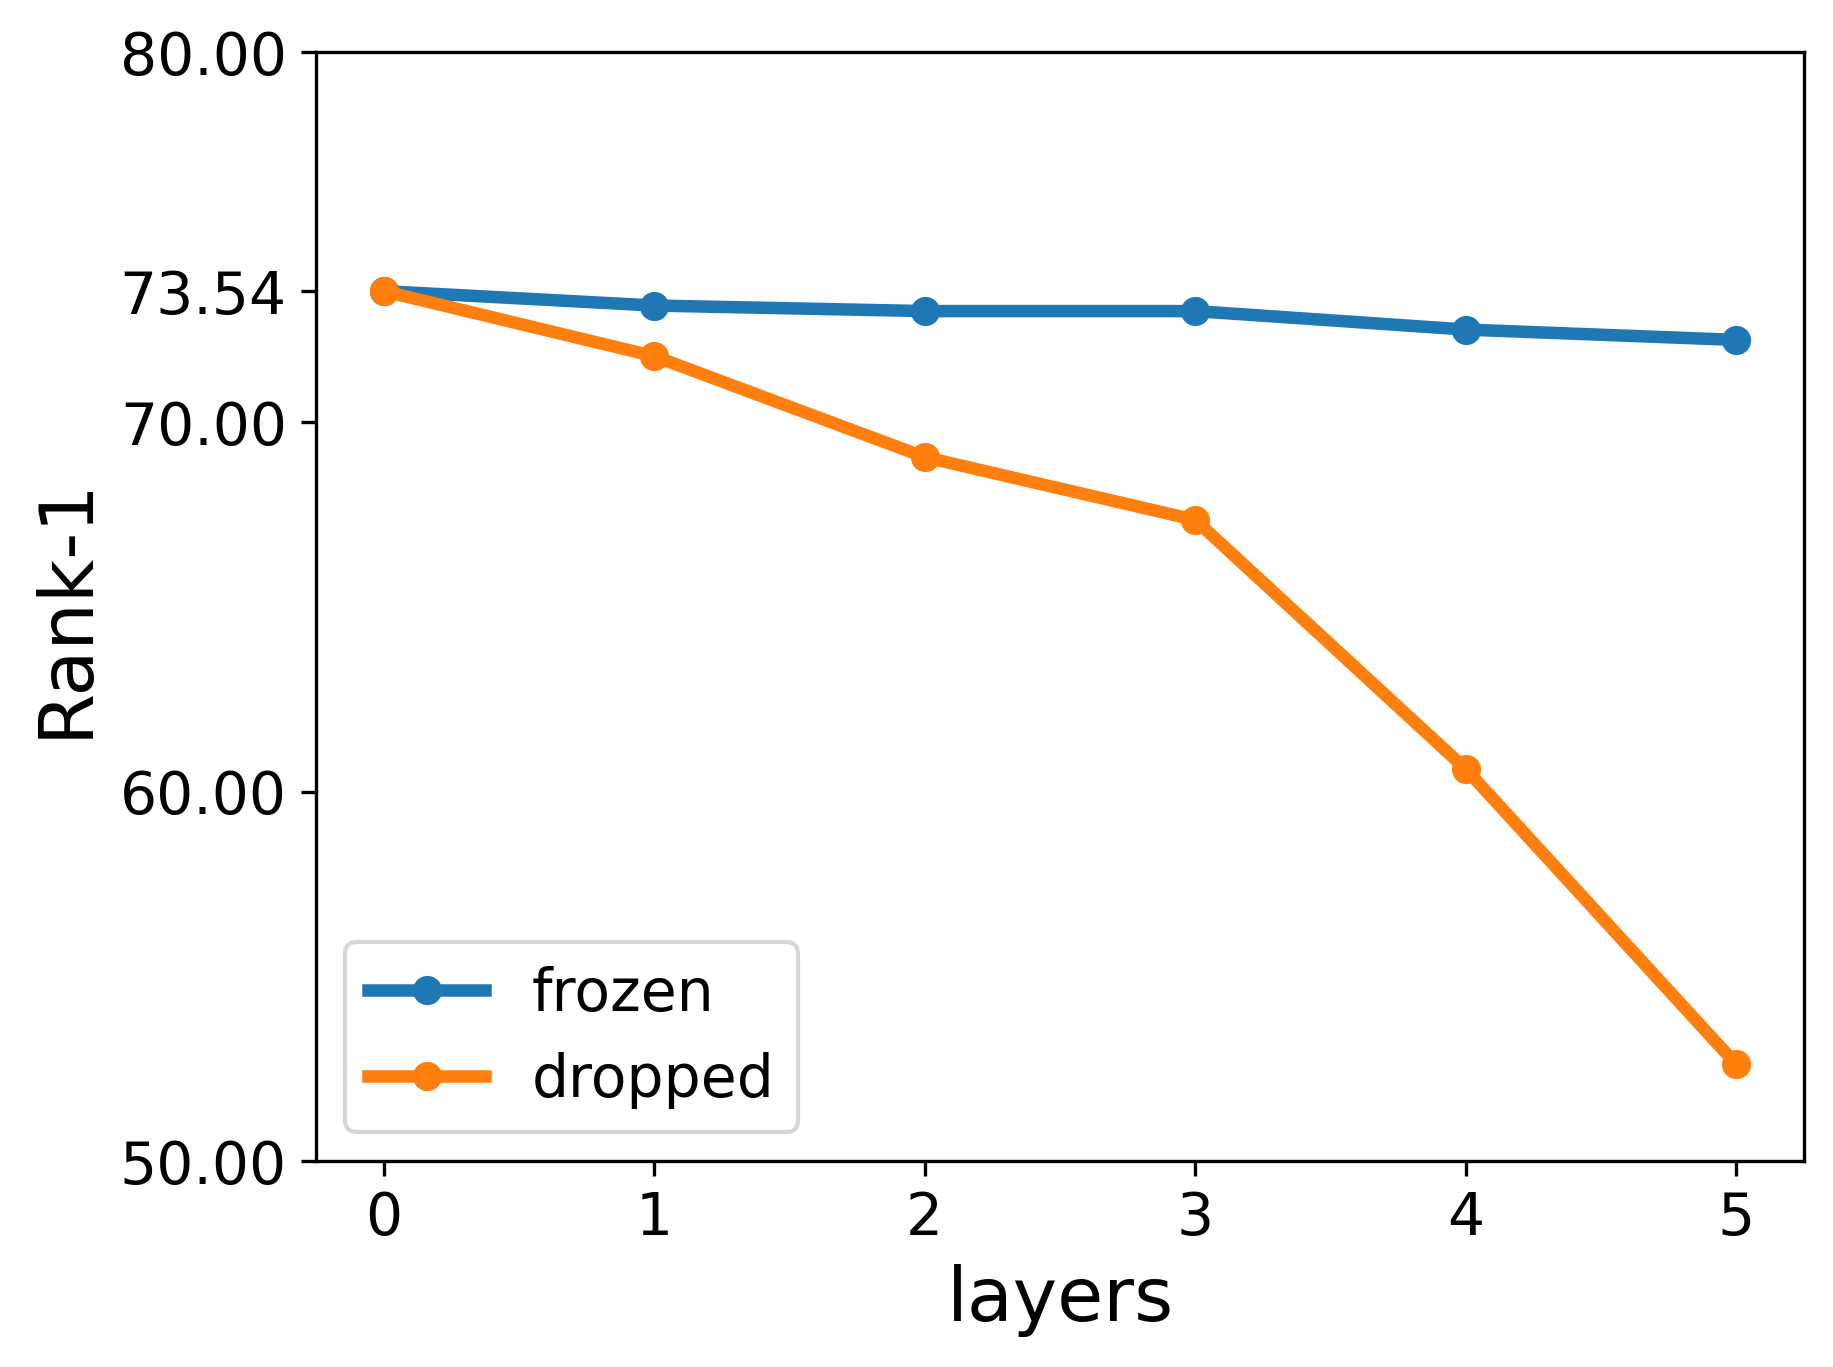
\includegraphics[width=0.48\columnwidth]{figures/original_plotimage.png}}
    \hspace{0.02\columnwidth}
    \subfloat[Simplified TBPS-CLIP]{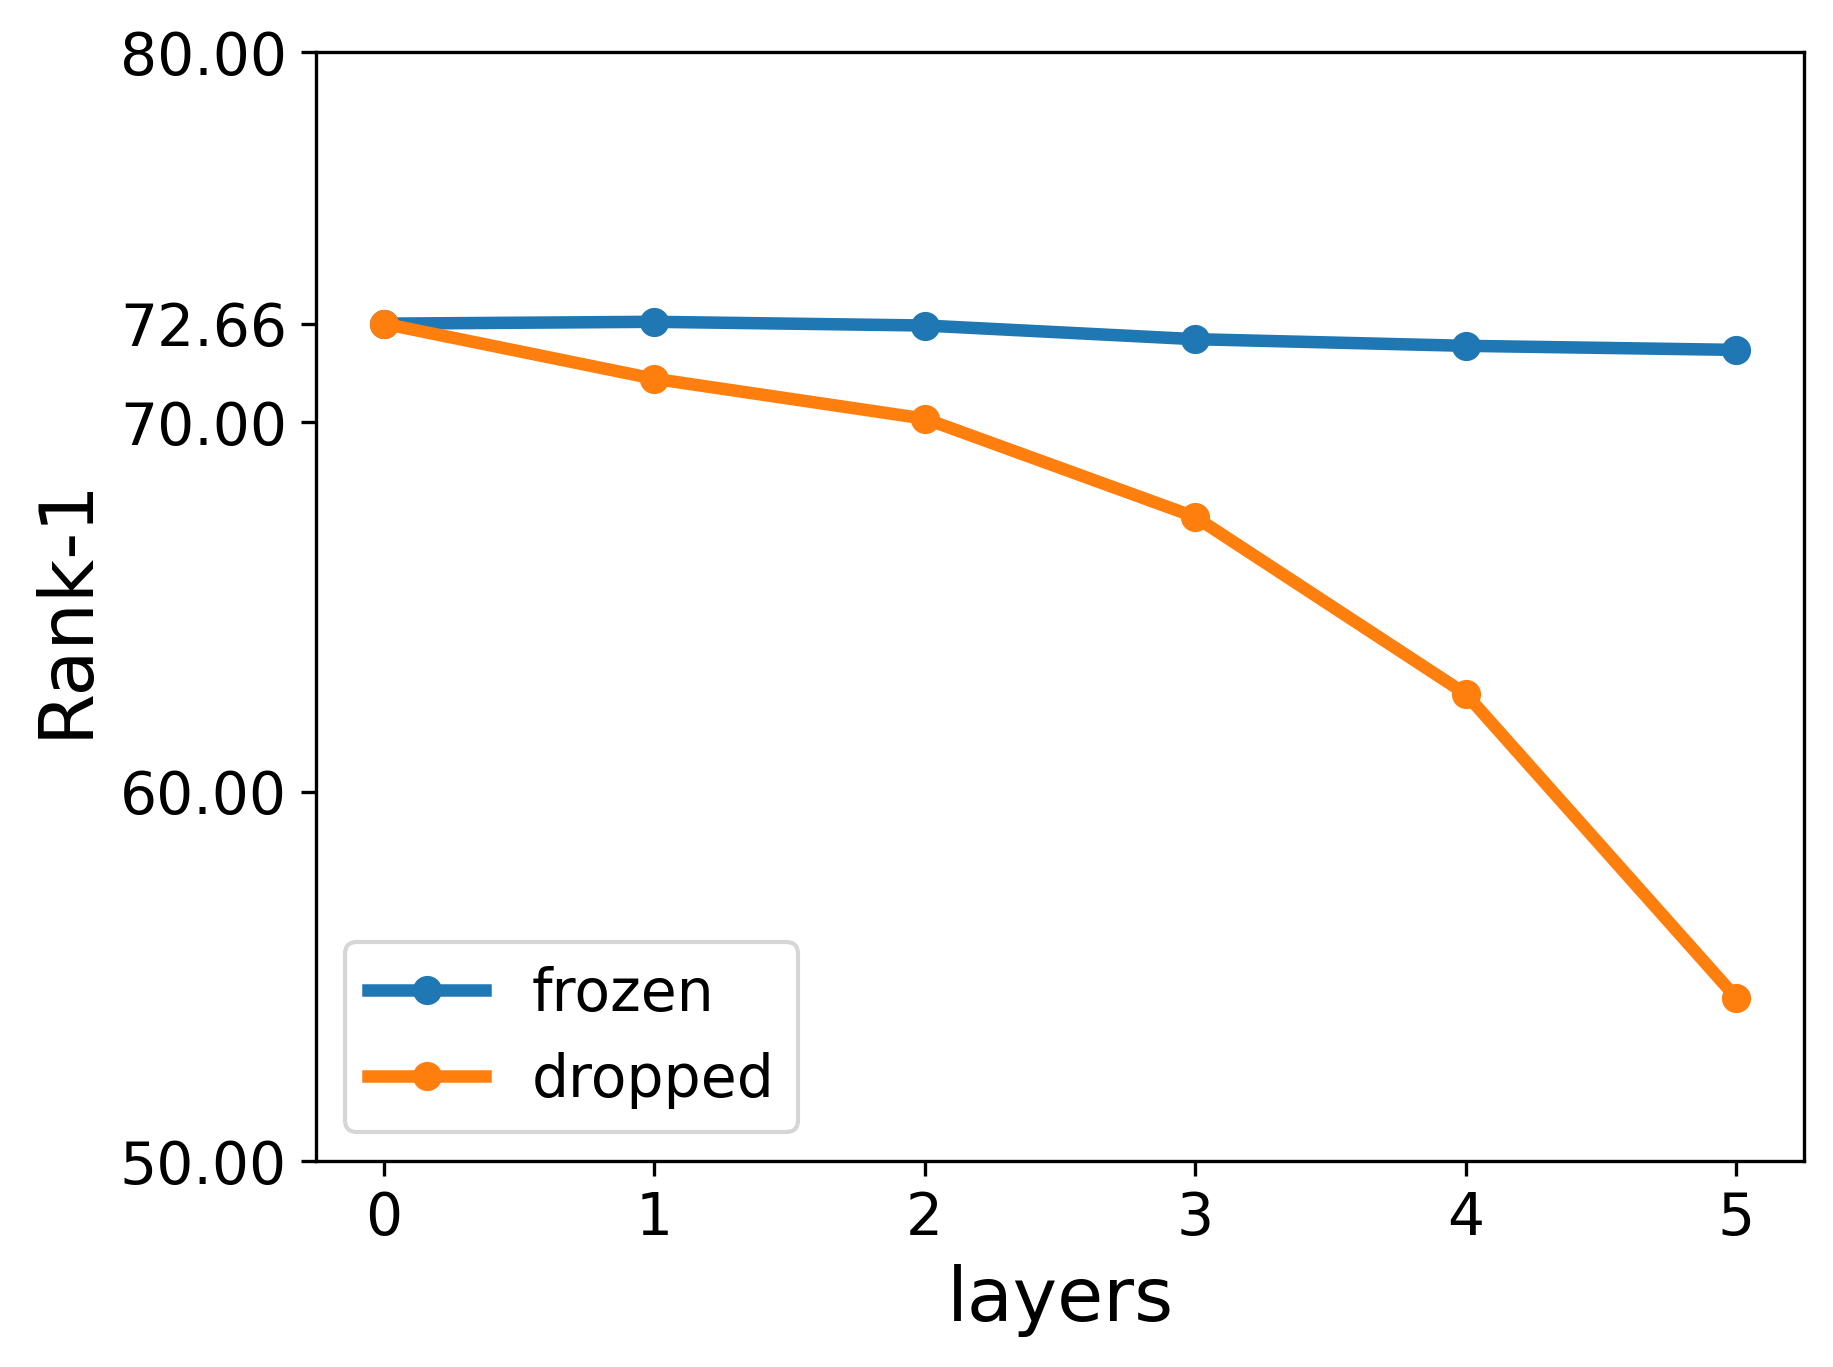
\includegraphics[width=0.48\columnwidth]{figures/simplified_plotimage.png}}
    \caption{The trend of performance when dropping/freezing some layers of the text encoder in the proposed TBPS-CLIP and simplified TBPS-CLIP.}
    \label{fig:plotimage}
    \vspace{-0.5cm}
\end{figure}

\begin{table}[t]
\setlength{\abovecaptionskip}{-0.01cm}
\begin{center}
{\caption{Performance under few-shot settings (5\% training data) on CUHK-PEDES.}\label{table:few_shot}}
\resizebox{0.47\textwidth}{!}{
\begin{tabular}{l!{\vrule}cccc}
\toprule
% \rule{0pt}{12pt}
Methods  & Rank-1 & Rank-5 & Rank-10 & mAP \\
\midrule
CLIP~\cite{radford2021learning} & 38.37 & 62.26 & 72.34 & 35.39 \\
CoOp~\cite{zhou2022learning} & 11.37 & 24.19 & 32.46 & 10.48 \\
CLIP-Adapter~\cite{gao2021clip} & 11.96  & 25.45  & 33.56  & 10.91  \\
\hdashline
TBPS-CLIP & 42.98 & 66.26 & 74.94 & 38.86 \\
Simplified TBPS-CLIP & 43.65 & 66.60 & 75.91 & 39.30 \\
\bottomrule
\end{tabular}}
\end{center}
\vspace{-0.5cm}
\end{table}

%To demonstrate the generalizability of our empirical study and make a fair comparison, additional experiments using ViT-B/16 besides ViT-B/32 as the image encoder are also conducted.

%In general, the methods using CLIP as the backbone outperform those without CLIP by a significant margin. Even the baseline on the ViT-B/16 image backbone with 65.37\% rank-1 accuracy performs on par with the best IVT among methods without CLIP, which has a rank-1 accuracy of 65.59\%.

%Among methods with CLIP, our proposed TBPS-CLIP performs on par with state-of-the-art method IRRA on CUHK-PEDES, but outperforms it by a margin on ICFG-PEDES and RSTPReid. Specifically, on CUHK-PEDES, TBPS-CLIP achieves 73.85\% Rank-1 accuracy, which is a minor gain over 73.38\% of IRRA, but has a slightly worse mAP of 65.62\%, compared with 66.13\%. On ICFG-PEDES, TBPS-CLIP achieves 65.01\% and 39.90\% for Rank-1 accuracy and mAP, respectively, with a gain of 1.55\% and 1.84\% over IRRA. On RSTPReid, The Rank-1 accuracy and mAP are 62.85\% and 48.44\%, exceeding IRRA by 2.65\% and 1.27\%.

%t is worth noting that since our ablation studies are carried out on CUHK-PEDES with a ViT-B/32 image backbone, the outstanding performances with ViT-B/16 on ICFG-PEDES and RSTPReid demonstrate that our method, without the need for designing specific modules, scales and generalizes well on different backbones and datasets.

\subsection{More Probing Experiments of TBPS-CLIP}

\subsubsection{Model Generalization.}
(1) We select IRRA~\cite{jiang2023cross}, the most advanced CLIP-based TBPS method so far, as the hotbed for verifying the generalization and effectiveness of TBPS-CLIP baseline.
Specifically, we adopt TBPS-CLIP (ViT-B/16) and its simplified version as the IRRA's baseline, respectively, instead of the original CLIP (ViT-B/16).
Table~\ref{table:genera} demonstrates the generalization and effectiveness of TBPS-CLIP.
\emph{More experimental results on other datasets are shown in the Appendix.}
(2) We study the few-shot capabilities (5\% training data) of TBPS-CLIP in Table~\ref{table:few_shot}, and \emph{more experimental results with 1\% training data and 10\% one are shown in the Appendix.}
CLIP presents a poor performance in few-shot TBPS, especially, the representative few-shot CLIP variants (CoOp and CLIP-Adapter) are even worse in performance.
The three methods are skilled in the few-shot image classification since the large-scale data knowledge of CLIP from the pre-training phase shares the same data characteristics as the downstream classification task.
However, TBPS is a fine-grained person-specific task and has a noticeable gap with the pre-trained data in CLIP.
The TBPS performance will be poor if there is insufficient training data to fine-tune CLIP,
and CoOp and CLIP-Adapter with the locked CLIP backbone in the fine-tuning phase also perform poorly in TBPS.
Alternatively, the proposed TBPS-CLIP with powerful learning capacity in TBPS can alleviate these problems and brings promising few-shot results.
More than that, the simplified TBPS-CLIP has superiority in the few-shot setting.

%The phenomenon contrasts strongly with that in other cross-modal tasks.The powerful cross-modal semantic learning capacity of CLIP from large-scale data knowledge in the pre-training phase naturally nourishes the downstream coarse-grained cross-modal tasks, all of which share the same data characteristics as the pre-trained data in CLIP.



% Optionally, we also conduct the experiments of adding IRRA modules (i.e., IRR, ID loss, etc.) to TBPS-CLIP baseline, or incorporating TBPS-CLIP modules (i.e., training tricks, various augmentations and losses, etc.) to IRRA. However, they do not fetch performance enhancement. TBPS-CLIP and IRRA are incompatible in code implementation due to different optimizes and optimization strategies and so on, thus the modules that have proven to be effective in one method may not be effective in another method and the explicit module blending of the two methods do not bring performance enhancement. It is expected that more ideas and works can be build directly on TBPS-CLIP in the future.

\subsubsection{Model Compression.}

% \begin{figure}
%   \centering
%   \begin{subfigure}[t]{1cm}
%     \centerline{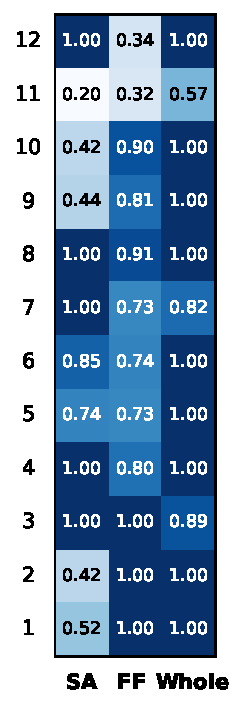
\includegraphics[width=\columnwidth]{figures/image_contribution.pdf}}
%     \caption{Co-attention}
%     \label{fig4:a}
%   \end{subfigure}
%   % \centering
%   % \begin{subfigure}[t]{0.3\linewidth}
%   %   \centerline{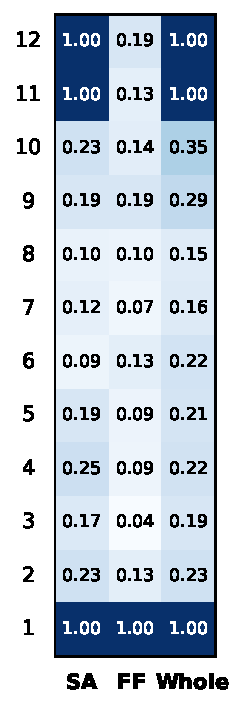
\includegraphics[width=\linewidth]{figures/text_contribution.pdf}}
%   %   \caption{Merged attention}
%   %   \label{fig4:b}
%   % \end{subfigure}

%   \caption{\textbf{Illustration of our multimodal interaction encoder and two other popular interaction modules.} (a) Co-attention, textual and visual features are fed into separate transformer blocks with self-attn and cross-attn independently to enable cross-modal interaction. (b) Merged attention, textual and visual features are concatenated together and then fed into a single transformer block. (c) Our multimodal interaction encoder, textual and visual features are first fused by a cross-attn layer and then fed into a single transformer block.}
%   \label{fig:importance}
% \end{figure}

We compute the two metrics of TBPS-CLIP in Section~\ref{sec:3.4} as the guidance for the model compression.
\emph{The computation of the metrics, the corresponding investigation of the internal properties of TBPS-CLIP, as well as the detailed explanation of model compression are shown in Appendix.}
Finally, from Figure~\ref{fig:plotimage}, we can clearly see that freezing some layers of the text encoder does not have much impact on performance while the dropping operation can negatively affect performance.
As a result, we can compress TBPS-CLIP during training by freezing part of text encoder.

\iffalse
\emph{We investigate the internal properties of TBPS-CLIP by two metrics $C^{\mathrm{1}}_i$ and $C^{\mathrm{2}}_i$ described in Section~\ref{sec:3.4} in the Appendix.
They guide the model compression.
%around CLIP for real-world TBPS applications in future.
Here we present as an example the compression of TBPS-CLIP (ViT-B/16) and simplified TBPS-CLIP (ViT-B/16), of which the detailed explanation is shown in the Appendix.}
From Figure~\ref{fig:plotimage}, we can clearly see that freezing some layers does not have much impact on performance while the dropping operation can negatively affect performance.
As a result, we can compress TBPS-CLIP during training by freezing part of text encoder.
\fi

%Figure~\ref{fig:importance} illustrates the importance of each module measured by the two metrics described in Section~\ref{sec:importance}. It is demonstrated that the two metrics are in good agreement with each other and reveal a common pattern. The pattern shows that for the text encoder, the top and bottom layers matter the most, indicating redundancy in the middle layers; the self-attention layers show more importance than feed-forward layers. In contrast, the contributions of different sub-layers in the image encoder are relatively evenly distributed. Consequently, removing any sub-layer in the model does not have a significant impact but results in a relatively consistent decrease in performance.



%The experimental results are illustrated in Table~\ref{table:few_shot}.
%When we directly apply the off-the-shelf pretrained CLIP to employ TBPS (\emph{i.e.}, zero-shot learning), the results are far from pretty, only reaching $8.98\%$ at Rank-1. It indicates that CLIP pre-trained in large-scale image-text data does not learn and capture fine-grained knowledge for TBPS, and also reveals the necessity of research on it. 
%When we adopt small amounts of data ($5\%$ of data samples) to fine-tune CLIP (\emph{i.e.}, few-shot learning), the performance improvement is reached and is also significant over in zero-shot setting, while still barely achieves $41.15\%$ at rank-1. Furthermore, we adopt two classical improved versions of CLIP for few-shot learning, \emph{i.e.}, CoOp and CLIP-Adapter, the slight performance enhancement is reached, and yet the retrieval results are still far from the current state of the art. 

%In our experiment setting, 5\% of data samples (\emph{i.e.} 1702 images and 3404 captions) in the training set of CUHK-PEDES are used for few-shot training. All the parameters of the model are updated in direct few-shot and CoOp, whereas only the parameters in the MLP head are trainable in CLIP-Adapter.

%As illustrated in Table~\ref{table:few_shot}, directly performing zero-shot retrieval on TBPS task behaves poor, only reaching 8.17\% rank-1 accuracy. As of few-shot performance, the improvement over zero-shot is significant, but still barely achieves 41.15\% rank-1 accuracy. CoOp and CLIP-Adapter both improves the performance over direct few-shot, but the enhancement is very small, with a gain of 0.57\% and 0.83\% rank-1 accuracy, respectively. In general, both zero-shot and few-shot performances are undesirable under TBPS; it could be assumed that many fine-grained details need to be identified in both image and text, which was not emphasized in the pre-training process of CLIP. Thus, fine-tuning with full data is demonstrated essential on TBPS for desirable performance.



\section{Conclusion}
% In this paper, empirical study is done utilizing CLIP for TBPS; a series training tricks and loss functions based on the CLIP framework are investigated to improve performance on TBPS task. Meanwhile, thorough and systematic study on data augmentation strategies on TBPS is carried out for the first time. A novel inverse KL loss, augmentation pool and ConcatGen are introduced at the same time. Consequently, with the studies above, our proposed TBPS-CLIP significantly boosts the performance from the vanilla CLIP and achieves state-of-the-art performance, without introducing any specifically designed module. In addition, preliminary exploration of zero/few-shot capability are tested; module importance of TBPS-CLIP is analyzed to provide a reference for model pruning and compression for real-world deployment. In general, our empirical study fully exploits the potential of CLIP but also provides insights of its internal property.
%It is expected to provide valuable references and insights for further VLP-based study in this community. 

This paper makes a thorough empirical study to explore the potential of CLIP for TBPS.
We empirically prove that CLIP, only equipped with some common data augmentations, loss functions, and practical training tricks (without introducing any sophisticated module), can achieve promising results on multiple TBPS benchmarks.
Further, we prove the effectiveness of the proposed TBPS-CLIP from two viewpoints: model generalization and model compression. 
The empirical study is expected to provide a practical guideline for future CLIP-based TBPS research.


% \bigskip
% \noindent Thank you for reading these instructions carefully. We look forward to receiving your electronic files!

\bibliography{aaai24}

% {\small
% \bibliographystyle{ieee_fullname}
% \bibliography{bibliography}
% }

\appendix
% \section{Appendix}

\section{Empirical Studies}

\subsection{Training Tricks}
\textbf{Global Gradients Back-propagation.}
In multi-GPU training scenarios, data parallelism is often employed to increase the batch size and thus enhance performance.
In such a case, a default practice of code implementation is to only back-propagate the gradient of the loss functions from a local GPU while discarding the gradients gathered from other GPUs. 
We experimentally observe a notable performance gain when back-propagating all gradients across GPUs.

\textbf{Dropout.}
As a regularization trick, dropout~\cite{srivastava2014dropout} is commonly employed by randomly setting some of the neurons' outputs to zero during model training.
In this study, we apply it to the self-attention modules of the text encoder empirically with a probability of $0.05$. 
%The dropout technique~\cite{srivastava2014dropout} randomly sets some of the neurons outputs to zero during the forward pass. As a regularization method, it is commonly employed in the training of sizable, deep neural networks to avert overfitting and enhance the model's generalization capabilities. In this study, We apply this technique to the multi-head self-attention mechanism and the input logits of the text encoder with a rate of 0.05.
% bycm：
% 1. 针对 We apply this technique to the multi-head self-attention mechanism and the input logits of the text encoder，应该是apply到什么模块，multi-head self-attention我理解，input logits是什么，怎么apply？建议写清楚点？另外，为什么仅针对text encoder呢？很突兀，论文是不是要提到？
% re: "input logits是什么，怎么apply"我的问题，input logits上是没有的，之前忘记删了。只用到text encoder上的原因我查一下之前的记录，如果是image那边效果不好的话那我加个empirically，还是再一句话说一下text那边效果好？
% 2. dropout~\cite{srivastava2014dropout}这里，如果篇幅够的话，建议多引用多加几个
% re: 最后看一下吧，估计篇幅比较难

\textbf{Locking Bottom Layers.}
When fine-tuning the model, a practical technique is to freeze a portion of the lower layers of the network or to assign them a reduced learning rate. In this study, we observe a slightly better performance when the first convolutional layer in the image encoder, which maps image patches to tokens, is locked.

\textbf{Soft Label.}
% To stabilize the training process, we draw inspiration from ALBEF~\cite{li2021align} and apply the soft label. Specifically, let $q_{i,j}$ denote the one-hot label which equals 1 if samples $i$ and $j$ are a positive pair, otherwise 0; the pseudo-label $q^\prime_{i,j}$ indicates the matching probability between samples $i$ and $j$ inferred by the model. The training label $\mathbf{q}_{i,j}$ is the averaged value of the one-hot label and pseudo-label, formulated as $\mathbf{q}_{i,j} = \frac{1}{2} (q_{i,j} + q^\prime_{i,j})$.
% 上面是带公式的版本，下面是不带公式的版本，我感觉不带公式的话，下面itc loss那里的表述也会更清楚
To stabilize the training process, we draw inspiration from ALBEF~\cite{li2021align} and apply the soft label to the loss function.
% Specifically, let the pseudo-label indicate the matching probability between the image and text output from the model, the soft label is the averaged value of the pseudo-label and ground-truth label.
Specifically, let the pseudo-label represent the matching probability between the image and text, as output from the model. The soft label is then the average value of the pseudo-label and ground-truth label.
% Specifically, the original one-hot label equals 1 if the image-text pair is a positive match, otherwise 0; 


\subsection{Data Augmentation}

\paragraph{Image Augmentation.}
The image augmentations are divided into removal and alteration groups, and their illustrations are presented in Figure~\ref{fig:img-aug}.

\begin{figure}
\setlength{\abovecaptionskip}{0.05cm}
\centerline{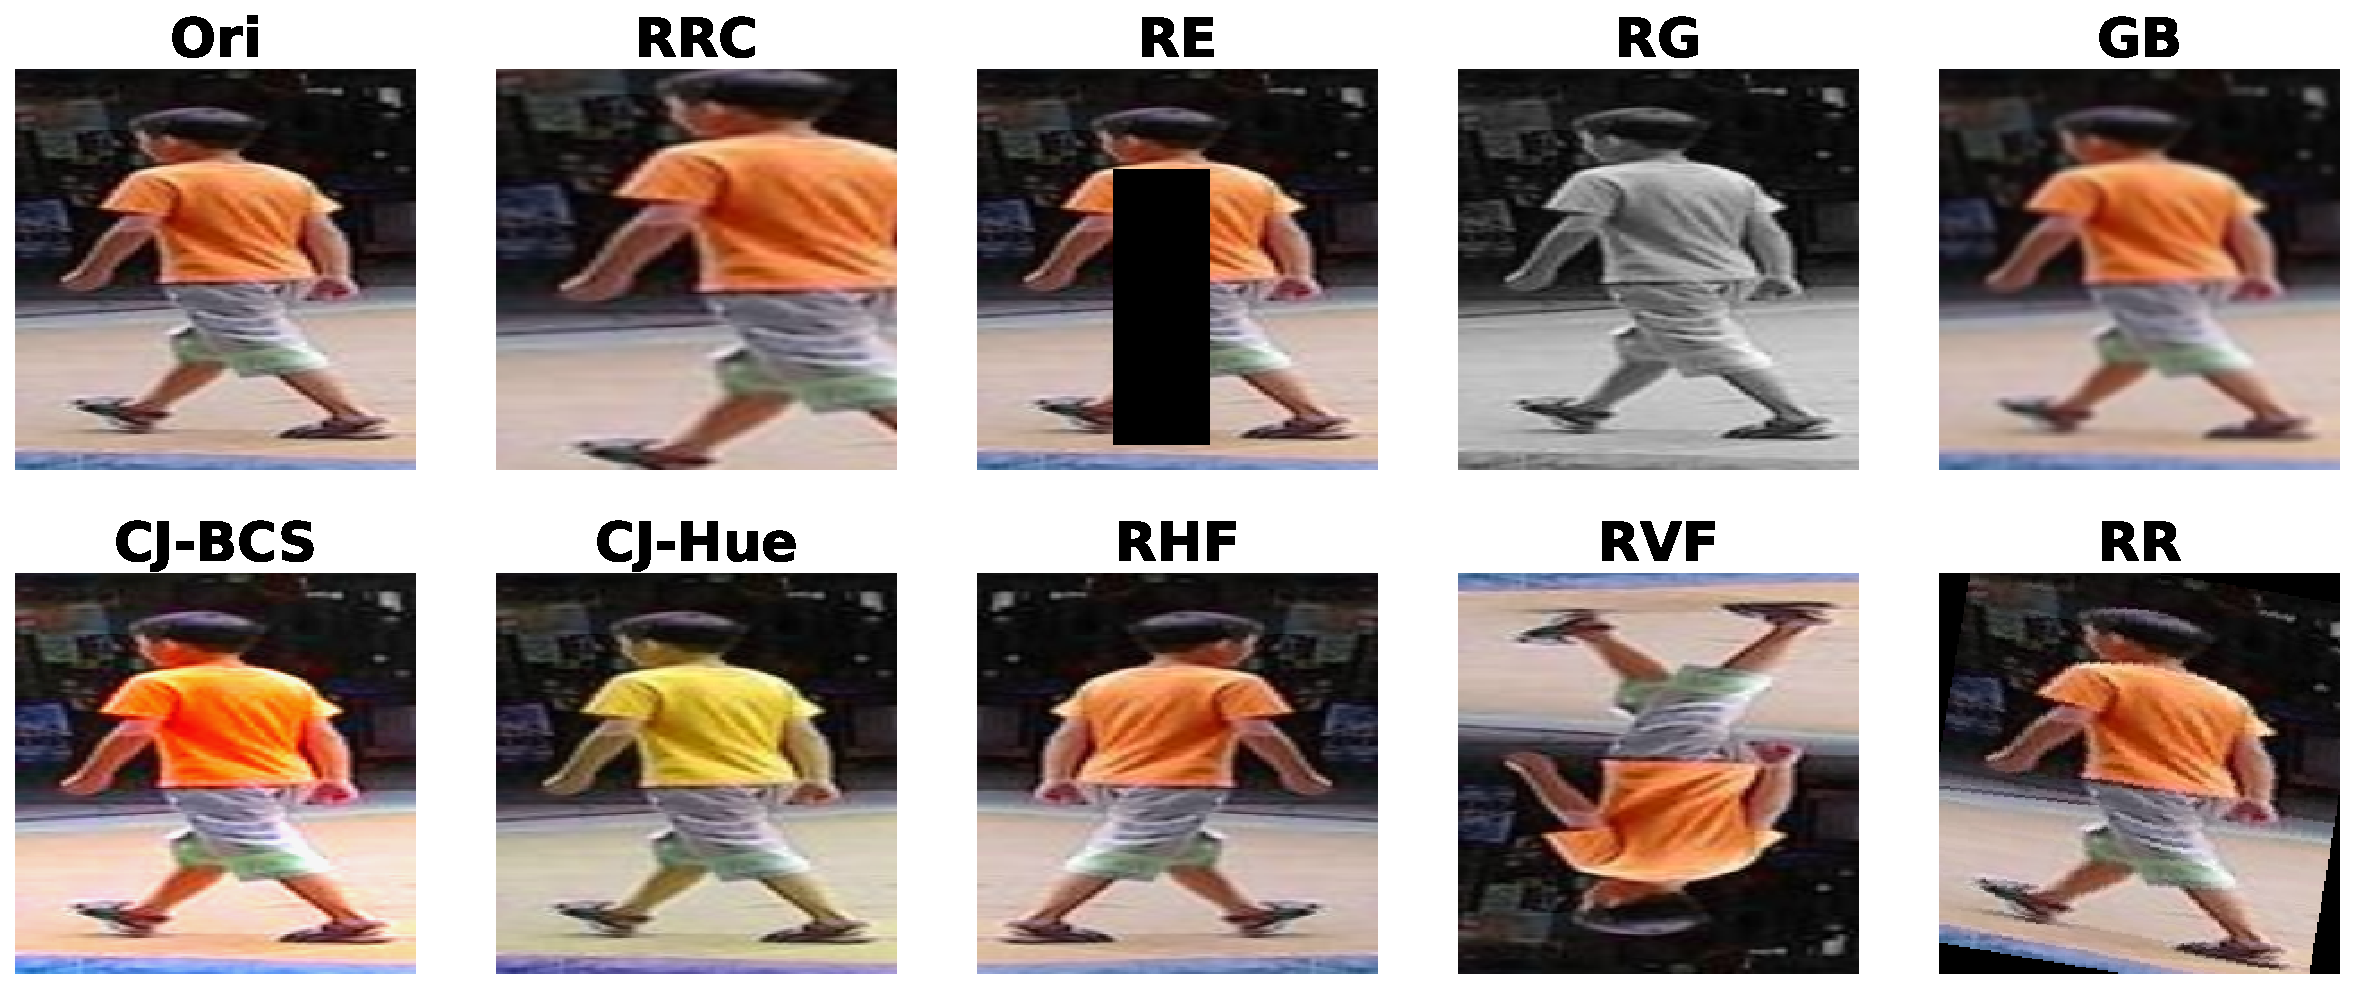
\includegraphics[width=0.98\columnwidth,height=0.52\linewidth]{figures/figure-aug.pdf}}
\caption{Illustration of the image and its augmented counterparts.
\textbf{Ori:} the original image. 
\textbf{RRC:} RandomResizedCrop. 
\textbf{RE:} RandomErasing. 
\textbf{RG:} RandomGrayscale. 
\textbf{GB:} GaussianBlur. 
\textbf{CJ-BCS:} ColorJitter with adjusted brightness, contrast and saturation. 
\textbf{CJ-Hue:} ColorJitter with adjusted hue. 
\textbf{RHF:} RandomHorizontalFlip. 
\textbf{RVF:} RandomVerticalFlip. 
\textbf{RR:} RandomRotation.} \label{fig:img-aug}
\vspace{-0.5cm}
\end{figure}

The group of removal has:
\begin{itemize}
    \item \textit{RandomResizedCrop} crops a random portion of an image, and then resizes it to a pre-set size as a new augmented image. 
    %For the cropping operation, the aspect ratio of the cropped area is randomly selected in $\left[ \frac{3}{4}, \frac{4}{3} \right]$ following the default setting in the PyTorch ecosystem, and the scale of the cropped area with respect to the original image is randomly chosen in $\left[ 0.9, 1 \right]$ during training. For the resizing operation, the augmented image size is $224 \times 224$.
    
    % The aspect ratio of the cropped area is randomly selected between (3/4, 4/3) (PyTorch default). The crop scale with respect to the original image is randomly chosen between $x$ and 1. This primarily removes information at the edge of an image.

    \item \textit{RandomErasing} erases a randomly selected rectangle within the image with a probability of $0.5$. 
    %The aspect ratio of the erased area is chosen stochastically between $\left[ \frac{3}{10}, \frac{10}{3} \right]$ following the default setting in PyTorch. The proportion of the erased area against the original image is selected randomly within the range $\left[ 0.02, 0.1 \right]$.

    \item \textit{RandomGrayscale} converts the inputted RGB image to a grayscale one with a probability of $0.1$, which can be interpreted as removing all the color information from the image.

    \item \textit{GaussianBlur} applies a Gaussian blur filter to the image, equal to removing its finer details while preserving the coarse content.
    %The Gaussian kernel size is set to 3, while the standard deviation $\sigma$ used for creating the kernel is randomly chosen between $\left[ \frac{1}{10}, 2 \right]$ following the default setting in PyTorch.
    
    % Standard deviation to be used for creating kernel to perform blurring. If float, sigma is fixed. If it is tuple of float (min, max), sigma is chosen uniformly at random to lie in the given range.
    % We fix the kernel size and adjust the range of $\sigma$, which determines the extent of the blur.
\end{itemize}

The group of alternation has:
\begin{itemize}
    \item \textit{ColorJitter} randomly adjusts the image's brightness, contrast, saturation, and hue. The brightness, contrast and saturation adjustments do not affect the image color, while the hue adjustment does. Thus, we have the former three grouped and studied, denoted as ColorJitter-BCS, while studying the hue separately, denoted as ColorJitter-Hue.
    %Consequently, we group the brightness, contrast and saturation together and have their strength tuned together, denoted as ColorJitter-BCS, and have the hue tuned separately, denoted as ColorJitter-Hue. Specifically, the strength of the group is denoted as $x_{cj1}$, and that of hue as $x_{cj2}$. The factor of bright brightness, contrast and saturation is chosen uniformly from $\left[ 1-x_{cj1}, 1+x_{cj1} \right]$, while the factor of hue is chosen uniformly from $\left[ -x_{cj2}, +x_{cj2} \right]$. $x_{cj1}$ and $x_{cj2}$ are both empirically set to $0.1$.
    % Consequently, we group the first three together and treat hue separately, adjusting the strength within each group.
    
    \item \textit{RandomHorizontalFlip} randomly flips the image horizontally with a probability of $0.5$.

    \item \textit{RandomVerticalFlip} randomly flips the image vertically with a probability of $0.5$.

    \item \textit{RandomRotation} rotates the image by an randomly angle.
    %chosen between $\left[ -15^{\circ}, +15^{\circ} \right]$.
\end{itemize}

\paragraph{Text Augmentation.}
We illustrate text augmentation in Table~\ref{table:txt-aug-demo}.

\begin{table}
\setlength{\abovecaptionskip}{-0.01cm}
\begin{center}
{\caption{Illustration of the text and its augmented texts.
\textbf{BT:} back translation.
\textbf{SR:} synonym replacement.
\textbf{RI:} random insertion.
\textbf{RS:} random swap.
\textbf{RD:} random deletion.}\label{table:txt-aug-demo}}
\resizebox{\columnwidth}{!}{
\begin{tabular}{c!{\vrule}p{6.0cm}}
\toprule
% \rule{0pt}{12pt}
Augmentations & Sentence \\
\midrule
None & a man with short black hair is wearing a white t-shirt, long black pants, red shoes and has a black book.\\
\midrule
BT & A man with a short black hair is wearing a white T-shirt, long black pants, red shoes, and black books.\\
\midrule
SR & a man with \textbf{brusk} black hair is wearing a white t-shirt, long black pants, red shoes and has a black \textbf{playscript}.\\
\midrule
RI & a man with short black hair is wearing a \textbf{weary} white t-shirt, long black pants, \textbf{fag out} red shoes and has a black book.\\
\midrule
RS & a \textbf{long} with short black hair is wearing a white t-shirt, \textbf{man} black \textbf{black} red shoes and has a \textbf{pants}, book.\\
\midrule
RD & a man with short black is wearing a \textbf{white} t-shirt, long black pants, red shoes and has a black book.\\
\bottomrule
\end{tabular}
}
\end{center}
\vspace{-0.5cm}
\end{table}


%For clarity, we illustrate all studied augmentations, including image augmentation in Figure~\ref{fig:img-aug}, pair augmentation in Figure~\ref{fig:pair-demo} and text augmentation in Table~\ref{table:txt-aug-demo}.

\subsection{Model Generalization}
We conduct the few-shot experiments to verify the model generalization.
Among them, two representative few-shot CLIP methods, CoOp~\cite{zhou2022learning} and CLIP-Adapter~\cite{gao2021clip}, are added for the performance comparison. 

%We conduct the empirical studies on two representative few-shot CLIP methods, CoOp~\cite{zhou2022learning} and CLIP-Adapter~\cite{gao2021clip}.

CoOp is a prompt-based method. It employs learnable vectors as soft text prompts, which are acquired by training small amounts of samples.
The original CLIP backbone is locked during training.
Specifically, the $M$ learnable tokens are prepended to the text, such that the input of the text encoder can be represented as:
\begin{equation}
    \text{Text} = [\text{V}]_1 [\text{V}]_2 \hdots [\text{V}]_M [\text{T}]_1 [\text{T}]_2 \hdots [\text{T}]_N,
\end{equation}
where $[\text{V}]_m$ ($m=1, \cdots, M$) is a learnable prompt vector and $[\text{T}]_n$ ($n=1, \cdots, N$) is the vector of the original text token.
The learnable prompt is experimentally initialized as `a pedestrian photo of'.
%$M$ is experimentally set to $1$ to obtain the best performance.
%$[\text{BOS}]$ and $[\text{EOS}]$ are tokens marking the beginning and end of the sentence, respectively. 
%The feature representations of all tokens share the same dimension. 

%Besides the prompt-based method CoOp, CLIP-Adapter demonstrates that fine-tuning a small portion of parameters can also achieve comparable or better results in the few-shot setting. Specifically, A two-layer MLP is appended to the text or image encoder in a residual connection manner and its parameters are trained based on small amounts of data, while the original backbone is locked to avoid training a large amount of parameters. The final representation $h^\prime$ can be formulated as:

%\footnote{We can append $\mathcal{G}$ on all image and text encoders, and yet better results are obtained by only appending on image encoder in CLIP-Adapter~\cite{gao2021clip}.}
CLIP-Adapter is an adapter-based method, in which a two-layer MLP $\mathcal{G}$ is appended on the image encoder of CLIP in a residual connection manner.
The parameters of $\mathcal{G}$ are trained based on small amounts of data, while the original backbone is locked.
The final representation $\hat{f}$ can be formulated as:
\begin{equation}
    \hat{f} = \alpha \mathcal{G}(f) + (1 - \alpha) f,
\end{equation}
where $\alpha$ is a residual factor and is experimentally set to $0.4$, and $f$ is the representation from the original model.


\subsection{Model Compression}
\label{MMC}
Two evaluation metrics~\cite{wang2020rethinking} are elaborated in detail here.
The first one estimates the contribution of a specific module by removing the module and observing the consequent performance drop.
Formally, let $\Delta{M}_i$ denotes the performance drop when the module $i$ is removed, and the contribution score of the module $i$ is defined as:
% \begin{equation}
%     Contri_i = \frac{\widehat{M}_i}{\widetilde{M}} ~~~ \text{where} ~~~ \widetilde{M} = \max\{\widehat{M}_i\},
% \end{equation}
\begin{equation}
    C^{\mathrm{1}}_i = \frac{\Delta{M}_i}{\max\{\Delta{M}_1, \dots, \Delta{M}_n\}},
    % ~~~ where ~~~ i \in n,
\end{equation}
where $n$ is the number of modules to be evaluated.
A higher $C^{\mathrm{1}}_i$ signifies a greater performance drop when the module is absent, indicating more contribution of this module to the final performance.
%to avoid exploding drop, $\Delta{M}_i$ is clipped between 0 and a constant $C$  to obtain $\widehat{\Delta{M}}_i$. $\widehat{\Delta{M}}_i$ is then normalized by dividing the maximum performance drop of all the modules.

The second metric probes the module's importance by measuring how closely the module's weights can close their initial values while maintaining a certain level of performance. Specifically, the contribution score of the module $i$ is defined as:
\begin{equation}
     C^{\mathrm{2}}_i = \min \alpha_i ~~~~  s.t. ~ M(\theta_i)-M(\theta_i^{\alpha_i}) < \epsilon,
     \label{eq:C2}
\end{equation}
where $\theta_i$ is the final optimized weights of the module $i$ and its corresponding model's performance is $M(\theta_i)$, and $\theta_i^{\alpha_i}= (1-\alpha_i)\theta_i^0 + \alpha_i \theta_i$ ($\alpha_i \in [0,1]$) represents a convex combination of the initial weights $\theta_i^0$ and final weights $\theta_i$ and its corresponding model's performance is $M(\theta_i^{\alpha_i})$.

%and $M(\theta_i)$ (\emph{resp.} $M(\theta_i^{\alpha_i})$) denotes the model's performance with the weights of the module $i$ being $\theta_i$ (\emph{resp.} $\theta_i^{\alpha_i}$).

A smaller $\alpha_i$ indicates that $\theta_i^{\alpha_i}$ is closer to the initial weights $\theta_i^0$.
Thus, a smaller $C^{\mathrm{2}}_i$ implies that the weights of the module $i$ can be moved from their final weights to randomly initialized ones, suggesting a lower contribution of the module to the model performance.

\begin{table}[t]
\setlength{\abovecaptionskip}{-0.01cm}
\begin{center}
{\caption{Ablation study of the hyperparameter on image augmentation on CUHK-PEDES. The underlined hyperparameter value is eventually used in the experiments.}\label{table:app-img-aug}}
% \begin{adjustbox}{max width=\textwidth}
\resizebox{\columnwidth}{!}{
\begin{tabular}{c!{\vrule}cc!{\vrule}ccc}
% \hline
\toprule
% \rule{0pt}{12pt}
Method & Hyperparameter & Value & Rank-1 & Rank-5 & mAP \\
% \hline
\midrule
% Baseline & \multicolumn{2}{c}{Modified CLIP} & 64.34 & 84.05 & 57.53 \\
% \midrule
\multirow{3}{*}{\shortstack{Random\\Resized\\Crop}} & \multirow{3}{*}{$x_{RRC}$} & $0.3$ & 64.82 & 84.94 & 58.33 \\
& & $0.6$ & 65.11 & 84.65 & 58.66 \\
& & \underline{${0.9}$} &  \underline{65.29} &  \underline{85.01} &  \underline{58.62} \\
\midrule
\multirow{3}{*}{\shortstack{Random\\Erasing}} & \multirow{3}{*}{$\left[x_{RE},y_{RE}\right]$} & $\left[0.02, 0.10\right]$ & 64.51 & 84.86 & 58.00 \\
& & $\left[{\underline{0.10}}, {\underline{0.20}}\right]$ &  \underline{64.64} &  \underline{84.34} &  \underline{58.08} \\
& & $\left[0.20, 0.30\right]$ & 64.30 & 84.60 & 57.97 \\
\midrule
% \multirow{3}{*}{\shortstack{ Random\\ Grayscale}} & \multirow{3}{*}{$p_{RG}$} & ${0.1}$ &  65.29 &  84.67 &  58.18 \\
% & & $0.3$ & 63.99 & 84.34 & 57.22 \\
% & & $0.5$ & 63.01 & 84.62 & 56.10 \\
% \midrule
\multirow{3}{*}{\shortstack{Gaussian\\Blur}} & \multirow{3}{*}{$k$} & $\underline{3}$ & \underline{55.30} & \underline{77.86} & \underline{49.82} \\
& & $7$ & 47.01 & 71.02 & 42.66 \\
& & $11$ & 46.48 & 70.60 & 42.09 \\
\midrule
% \multirow{3}{*}{\shortstack{Color\\Jitter-BCS}} & \multirow{3}{*}{$x_{cj1}$} & ${0.1}$ &  64.86 &  84.65 &  57.85 \\
% & & $0.2$ & 64.72 & 84.24 & 57.50 \\
% & & $0.4$ & 64.23 & 84.73 & 57.52 \\
% \midrule
% \multirow{3}{*}{\shortstack{Color\\Jitter-Hue}} & \multirow{3}{*}{$x_{cj2}$} & $0.1$ & 64.12 & 84.81 & 57.41\\
% &&$0.2$ & 63.86 & 84.02 & 56.66\\
% &&$0.4$ & 63.69 & 84.11 & 57.08\\

\multirow{6}{*}{\shortstack{Color\\Jitter}} & \multirow{3}{*}{$x_{cj1}$} & ${\underline{0.1}}$ &  \underline{64.86} & \underline{84.65} & \underline{57.85} \\
& & $0.2$ & 64.72 & 84.24 & 57.50 \\
& & $0.4$ & 64.23 & 84.73 & 57.52 \\
\cmidrule{2-6}
 & \multirow{3}{*}{$x_{cj2}$} & $\underline{0.1}$ & \underline{64.12} & \underline{84.81} & \underline{57.41}\\
&&$0.2$ & 63.86 & 84.02 & 56.66\\
&&$0.4$ & 63.69 & 84.11 & 57.08\\
% \cmidrule{2-6}
\midrule
%  RHF & $p_{RHF}$ & $0.5$ &  65.48 &  84.86 &  58.46 \\
% \midrule
% RVF & $p_{RVF}$ & $0.5$ & 64.65 & 84.36 & 57.80 \\
% \midrule
\multirow{3}{*}{\shortstack{Random\\Rotation}} & \multirow{3}{*}{$degrees$} & $7.5$ & 65.42 & 85.53 & 58.57 \\
& & ${\underline{15}}$ &  \underline{65.50} &  \underline{85.20} &  \underline{58.92} \\
& & $30$ & 65.06 & 84.99 & 58.45 \\
% \hline
\bottomrule
% \rule{0pt}{5pt}
% \multicolumn{6}{l}{\multirow{2}{*}{\shortstack{RHF: RandomHorizontalFlip. RVF: RandomVerticalFlip. \\The $bcs$ parameter of ColorJitter represents brightness, contrast and saturation.}}}
\end{tabular}}
% \end{adjustbox}
\end{center}
\vspace{-0.5cm}
\end{table}


\section{Experiments}

\paragraph{Datasets.}
\textbf{CUHK-PEDES}~\cite{li2017person} is the first TBPS dataset published in $2017$ and the most widely used. This dataset has an average of $3$ images per person, and $2$ textual descriptions accompany each image. They are divided into a train set with $34,054$ images of $11,003$ identities, a validation and a test set containing $3,078$ and $3,074$ images of $1,000$ identities, respectively.
\textbf{ICFG-PEDES}~\cite{ding2021semantically} is a larger dataset that contains a train set with $34,674$ image-text pairs of $3,102$ identities and a test set with $19,848$ image-text pairs of $1,000$ identities. The images include more complex backgrounds and illumination, and the text description is longer.
\textbf{RSTPReid}~\cite{zhu2021dssl} is a newly published dataset for suitably handling real scenarios. Each identity has $5$ images captured by different cameras, and each image corresponds to $2$ textual descriptions in this dataset. All are split into three training, validation and test subsets with $3,701$, $200$ and $200$ identities, respectively.

\paragraph{Evaluation Metrics.}
The commonly used Rank-$k$ metric and mean Average Precision (mAP) are adopted as the metrics to evaluate the performance in our experiments. Rank-$k$ demonstrates that at least one correct match is retrieved among results within top $k$ similarities and $k$ is set to $1$, $5$ and $10$ following the common practice. 

\paragraph{Implementation Details.} 
All experiments are conducted on 4 Nvidia A40 GPUs.
The $224 \times 224$ image is divided into $49$ patches with a size of $32 \times 32$ and are inputted to the model (ViT-B/32), and is divided with $16 \times 16$ in the model (ViT-B/16).
The texts with a fixed length of $77$ are inputted to the model.
The AdamW optimizer is employed with a linear warmup and cosine decay schedule, with $1e-6$, $5e-6$ and $1e-4$ for the initial, final and peak learning rate, respectively.
The model is trained for merely 5 epochs. 


%The illustrations of common image augmentations studied by us are shown in Figure~\ref{fig:img-aug}. Suppose that the original image is already resized to $224 \times 224$.

%the original sentence and the augmented sentences using the text augmentation strategies studied by us are listed in Table~\ref{table:txt-aug-demo}.


%The augmented image-text pair using MixGen and our proposed ConcatGen are displayed in Figure~\ref{fig:pair-demo}. Note that only images are shown since for text the captions are simply concatenated.
\iffalse
\begin{figure}
    \centering
    \subfloat[MixGen]{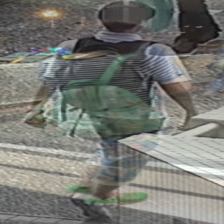
\includegraphics[width=0.28\columnwidth]{figures/mixgen_image.png}}
    \hspace{0.06\columnwidth}
    \subfloat[ConcatGen]{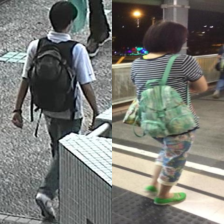
\includegraphics[width=0.3\columnwidth]{figures/mixgen_cat_image.png}}
    \caption{Illustration of pair augmentation. Note that only images are shown since the captions are simply concatenated for the text.}
    \label{fig:pair-demo}
\end{figure}
\fi

\subsection{Ablations of Data Augmentation}
% There are hyperparameters in several augmentations.
% They control to which extent the augmented data deviate from the original one. These hyperparameters studied in this work are described in this section.
The hyperparameters of data augmentation are described as follows.

\subsubsection{Image Augmentation}

% The group of removal has:
\begin{itemize}
    \item \textit{RandomResizedCrop.} For the cropping operation, the aspect ratio of the cropped area is randomly selected in $\left[ \frac{3}{4}, \frac{4}{3} \right]$ (default setting on Pytorch), and the scale of the cropped area with respect to the original image is randomly chosen in $\left[ x_{RRC}, 1 \right]$. The augmented image is then resized to $224 \times 224$. 
    %As shown in Table~\ref{table:app-img-aug}, a larger value of $x_{RRC}$ contributes to better performance and vice versa, which is reasonable. A small $x_{RRC}$ means a great possibility of image information loss and directly affects the performance. We experimentally set $x_{RRC}=0.9$.

    \item \textit{RandomErasing.} The aspect ratio of the erased area is randomly chosen in $\left[ \frac{3}{10}, \frac{10}{3} \right]$. The proportion of the erased area against the original image is selected randomly within the range $\left[ x_{RE}, y_{RE} \right]$. 
    %As shown in Table~\ref{table:app-img-aug}, RandomErasing with the relatively small erasion proportion ($\leq 0.30$) leads to the results without big changes and we experimentally set $\left[ x_{RE}, y_{RE} \right]=\left[ 0.10, 0.20 \right]$.

    \item \textit{GaussianBlur.} The size of Gaussian kernel is set to $k$, while the standard deviation is randomly chosen between $\left[ \frac{1}{10}, 2 \right]$.
% \end{itemize}


% The group of alternation has:
% \begin{itemize}
    \item \textit{ColorJitter.}
    % In ColorJitter, the brightness, contrast and saturation adjustments do not affect the image color, while the hue adjustment does.
    % Consequently, we group the brightness, contrast and saturation together, denoted as ColorJitter-BCS, and tune their strength using the same hyperparameter; the hue is tuned separately, denoted as ColorJitter-Hue. 
    % Specifically, the strength of the group is denoted as $x_{cj1}$, and that of hue as $x_{cj2}$. 
    The factor of bright brightness, contrast and saturation is chosen uniformly from $\left[ 1-x_{cj1}, 1+x_{cj1} \right]$, while the factor of hue is chosen uniformly from $\left[ -x_{cj2}, +x_{cj2} \right]$. 
    % $x_{cj1}$ and $x_{cj2}$ are both empirically set to $0.1$.

    \item \textit{RandomRotation.} The rotation degree is randomly chosen between $\left[ -degree, +degree \right]$.
\end{itemize}

We show the results of applying image augmentation with different hyperparameters mentioned above in Table~\ref{table:app-img-aug}.


\begin{table}[t]
\setlength{\abovecaptionskip}{-0.01cm}
\begin{center}
{\caption{Ablation study of the hyperparameter on text augmentation on CUHK-PEDES. The underlined hyperparameter value is eventually used in the experiments.}\label{table:app-txt-aug}}
% SR: synonym replacement. RI: random insertion. RS: random swap. RD: random deletion.
\resizebox{0.45\textwidth}{!}{
\begin{tabular}{c!{\vrule}c!{\vrule}cccc}
\toprule
% \rule{0pt}{12pt}
Method & $\alpha$ & Rank-1 & Rank-5 & Rank-10 & mAP \\
\midrule
\multirow{3}{*}{\shortstack{Back\\Translation}} & 0.05 & 64.31 & 84.39 & 90.48 & 57.43 \\
& \underline{ 0.1} & \underline{ 64.77} &  \underline{84.67} & \underline{ 90.56} &  \underline{57.49} \\
& 0.2 & 64.47 & 84.58 & 90.64 & 57.27 \\
\midrule
\multirow{3}{*}{\shortstack{Synonym\\Replacement}} & \underline{0.05} & \underline{63.95} & \underline{83.76} & \underline{89.96} & \underline{56.90} \\
& 0.1 & 61.45 & 81.47 & 88.16 & 54.98 \\
& 0.2 & 59.70 & 81.16 & 87.61 & 53.66 \\
\midrule
\multirow{3}{*}{\shortstack{Random\\Insertion}} & \underline{0.05} & \underline{63.71} & \underline{84.29} & \underline{90.03} & \underline{56.77} \\
& 0.1 & 62.83 & 83.17 & 89.49 & 56.06 \\
& 0.2 & 60.09 & 82.44 & 88.84 & 54.17 \\
\midrule
\multirow{3}{*}{\shortstack{Random\\Swap}} & \underline{0.05} & \underline{56.41} & \underline{79.08} & \underline{86.14} & \underline{49.29} \\
& 0.1 & 51.06 & 74.72 & 83.16 & 45.16 \\
& 0.2 & 49.51 & 73.31 & 81.95 & 43.74 \\
\midrule
\multirow{3}{*}{\shortstack{Random\\Deletion}} &  \underline{0.05} & \underline{65.53} & \underline{84.70} & \underline{90.87} & \underline{57.90} \\
& 0.1 & 64.99 & 85.19 & 90.37 & 57.33 \\
& 0.2 & 64.31 & 83.43 & 90.09 & 56.65 \\
\midrule
\multirow{3}{*}{\shortstack{EDA}} & \underline{0.05} & \underline{63.43} & \underline{83.77} & \underline{90.27} & \underline{56.15} \\
& 0.1 & 62.17 & 82.47 & 88.84 & 54.40 \\
& 0.2 & 60.66 & 81.45 & 88.27 & 53.50 \\
\bottomrule
% \multicolumn{6}{c}{\multirow{2}{*}{\shortstack{SR: synonym replacement. RI: random insertion. \\RS: random swap. RD: random deletion.}}}
\end{tabular}
}
\end{center}
\vspace{-0.5cm}
\end{table}

\subsubsection{Text Augmentation}
Following EDA~\cite{wei2019eda}, for \emph{synonym replacement}, \emph{random insertion} and \emph{random swap}, the process is repeated $\alpha L$ times in a sentence, where $L$ denotes the sentence length and $\alpha$ is a hyperparameter indicating the proportion of word modification. \emph{Random deletion} is applied with a probability of $\alpha$.
When applying \emph{back translation}, each sentence is replaced by the back translated one with a probability of $\alpha$.

The influence of the hyperparameter on performance is shown in Table~\ref{table:app-txt-aug}.

% In our experimental setup, French is adopted as the intermediate language as French has a relatively closer form to English, thus introducing less semantic change to the translated back text compared to most languages. Each sentence is replaced with the back translated one with a probability of $p_{BT}$ during training.


%\section{Ablation Study on Data Augmentation Hyperparameters}
%The influence of hyperparameters of image and text augmentations on CUHK-PEDES~\cite{li2017person} are shown in Table~\ref{table:app-img-aug} and Table~\ref{table:app-txt-aug}, respectively. 
% The optimal hyperparameters are highlighted in bold.

% \subsection{Image Augmentation}
% As shown in Table~\ref{table:app-img-aug}, the hyperparameters of image augmentations

\subsection{More Probing Experiments of TBPS-CLIP}

\subsubsection{Model Generalization.}
(1) We adopt the proposed TBPS-CLIP (ViT-B/16) and its simplified version as the IRRA's baseline, respectively.
Table~\ref{table:genera} shows the results on ICFG-PEDES and RST-PReid, which strongly verify the generalization and effectiveness of TBPS-CLIP.
(2) Table~\ref{table:few_shot} shows the few-shot results of several methods, including 1\% training data and 10\% training data, respectively.
The proposed TBPS-CLIP presents the absolute advantage under various few-shot settings.
Specifically, the simplified version is more competitive in performance.

\begin{table}
\setlength{\abovecaptionskip}{-0.01cm}
\begin{center}
{\caption{Results for applying the proposed TBPS-CLIP as the baseline of other method. The mean Inverse Negative Penalty(mINP) metric is used in IRRA and also adopted here for comparison.}\label{table:genera}}
\resizebox{0.49\textwidth}{!}{
\begin{tabular}{l!{\vrule}l!{\vrule}ccccc}
\toprule
Methods & Baselines & Rank-1 & Rank-5 & Rank-10 & mAP & mINP \\
\midrule
\multicolumn{7}{l}{\textit{ICFG-PEDES}} \\
\midrule
IRRA & CLIP & 63.46	& 80.25	& 85.82	& 38.06	& 7.93 \\
IRRA$^*$ & TBPS-CLIP & 65.64 & 81.25 & 86.61 & 40.77 & 9.36 \\
IRRA$^*$ & Simplified TBPS-CLIP & 64.90 & 80.95 & 86.48 & 40.50 & 9.40 \\
\midrule
\multicolumn{7}{l}{\textit{RST-PReid}} \\
\midrule
IRRA & CLIP & 60.20 & 81.30 & 88.20 & 47.17 & 25.28 \\
IRRA$^*$ & TBPS-CLIP & 63.40 & 82.60 & 89.00 & 49.45 & 26.78 \\
IRRA$^*$ & Simplified TBPS-CLIP & 62.35 & 82.00 & 87.90 & 49.82 & 27.41 \\
\bottomrule
\end{tabular}
}
\end{center}
\vspace{-0.1cm}
\end{table}

\begin{table}
\setlength{\abovecaptionskip}{-0.01cm}
\begin{center}
{\caption{Performance under few-shot settings on CUHK-PEDES.}\label{table:few_shot}}
\resizebox{0.47\textwidth}{!}{
\begin{tabular}{l!{\vrule}cccc}
\toprule
% \rule{0pt}{12pt}
Methods  & Rank-1 & Rank-5 & Rank-10 & mAP \\
\midrule
\multicolumn{5}{l}{\textit{1\% training data:}} \\
\midrule
CLIP~\cite{radford2021learning} & 27.84 & 49.51 & 60.56 & 25.88 \\
CoOp~\cite{zhou2022learning} & 10.98 & 23.98 & 31.50 & 10.22 \\
CLIP-Adapter~\cite{gao2021clip} & 11.22 & 24.22 & 31.71 & 10.30 \\
\hdashline
TBPS-CLIP & 27.94 & 51.20 & 62.07 & 27.60 \\
Simplified TBPS-CLIP & 30.05 & 51.56 & 62.23 & 28.53 \\
\midrule
\multicolumn{5}{l}{\textit{10\% training data:}} \\
\midrule
CLIP~\cite{radford2021learning} & 42.37 & 66.13 & 75.31 & 38.20  \\
CoOp~\cite{zhou2022learning} &  12.10 & 25.55 & 33.97 & 10.96  \\
CLIP-Adapter~\cite{gao2021clip} & 12.61 & 27.19 & 35.32 & 11.77 \\
\hdashline
TBPS-CLIP & 49.19 & 71.98 & 80.46 & 43.81 \\
Simplified TBPS-CLIP & 50.26 & 72.51 & 80.28 & 44.28 \\
\bottomrule
\end{tabular}}
\end{center}
\vspace{-0.5cm}
\end{table}

\begin{table}[t]
\setlength{\abovecaptionskip}{-0.01cm}
\begin{center}
{\caption{The ID of the dropped/frozen layers in the text encoder, and the corresponding number of the trainable parameters.}\label{table:layer-ID}}
\resizebox{0.43\textwidth}{!}{
\begin{tabular}{l!{\vrule}cccc}
\toprule
% \rule{0pt}{12pt}
\multirow{2}{*}{Layers} & \multirow{2}{*}{ID} & \multicolumn{2}{c}{Trainable Parameters} \\
 & & TBPS-CLIP & Simplified TBPS-CLIP \\
\midrule
0 & - & 149.2 & 149.0 \\
1 & 7 & 146.0 ($\downarrow{2\%}$) & 145.9 ($\downarrow{2\%}$) \\
2 & 7,8 & 142.9 ($\downarrow{4\%}$) & 142.7 ($\downarrow{4\%}$) \\
3 & 3,7,8 & 139.7 ($\downarrow{6\%}$) & 139.6 ($\downarrow{6\%}$)\\
4 & 3,5,7,8 & 136.6 ($\downarrow{8\%}$) & 136.4 ($\downarrow{8\%}$)\\
5 & 3,5,6,7,8 & 133.4 ($\downarrow{11\%}$) & 133.3 ($\downarrow{11\%}$)\\
\bottomrule
\end{tabular}
}
\end{center}
\vspace{-0.1cm}
\end{table}

\subsubsection{Model Compression.}


\begin{figure}[t]
\setlength{\abovecaptionskip}{0.08cm}
    \centering
    % \subfloat[Ablating unimportant components]{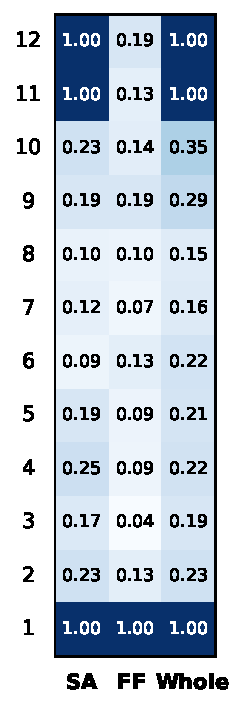
\includegraphics[width=0.45\textwidth]{figures/text_contribution.pdf}}
    % \hspace{0.03\textwidth}
    \subfloat[Txt enc. $C^\mathrm{1}_i$]{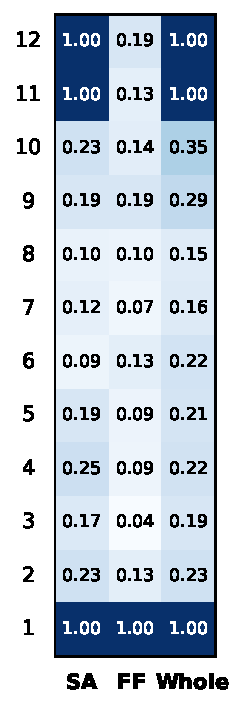
\includegraphics[width=0.25\columnwidth,height=0.36\textwidth]{figures/text_contribution.pdf}}
    % \hspace{0.003\textwidth}
    \subfloat[Txt enc. $C^{\mathrm{2}}_i$]{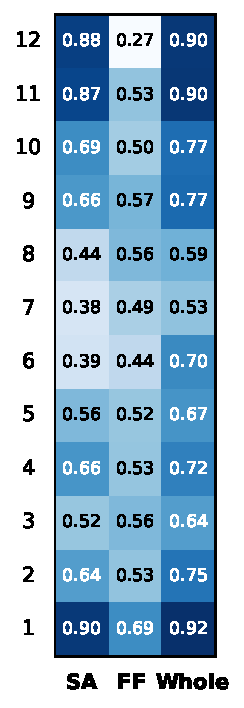
\includegraphics[width=0.25\columnwidth,height=0.36\textwidth]{figures/text_criticality.pdf}}
    % \hspace{0.003\textwidth}
    \subfloat[Img enc. $C^\mathrm{1}_i$]{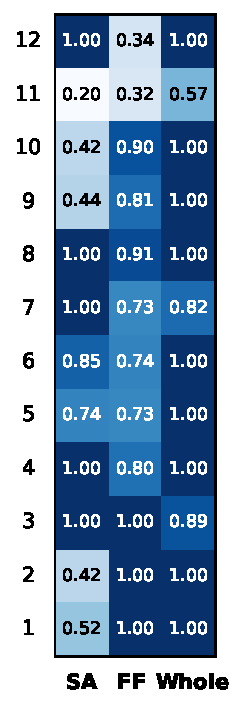
\includegraphics[width=0.25\columnwidth,height=0.36\textwidth]{figures/image_contribution.pdf}}
    % \hspace{0.003\textwidth}
    \subfloat[Img enc. $C^{\mathrm{2}}_i$]{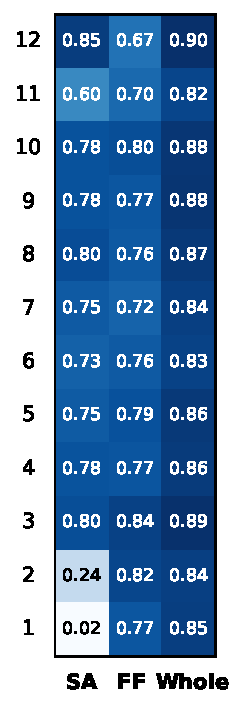
\includegraphics[width=0.25\columnwidth,height=0.36\textwidth]{figures/image_criticality.pdf}}
    \caption{Contributions of each module in the image encoder (Img enc.) and text encoder (Txt enc.) of TBPS-CLIP on CUHK-PEDES. SA: self-attention module. FF: feed-forward module. Whole: a whole layer in transformer.}
    \label{fig:importance}
    \vspace{-0.5cm}
\end{figure}

The proposed TBPS-CLIP has the same architecture as CLIP, in which there are a text encoder and an image one, both with 12 layers of transformer and each layer consists of one self-attention module and one feed-forward module.
Although it is already a lightweight architecture compared to other TBPS methods, we also consider its model compression for more convenient application in the industry.

We first explore the internal properties and functionalities of TBPS-CLIP by computing the contribution score of each module with the aid of two metrics $C^{\mathrm{1}}_i$ and $C^{\mathrm{2}}_i$ in Section~\ref{MMC}, in which we select the Rank-1 as the performance assessment and set $\epsilon$ to $3$ in the metric $C^{\mathrm{2}}_i$.

As shown in Figure~\ref{fig:importance}, (1)  the results of the two metrics are in good agreement with each other and reveal a common pattern; (2) for the text encoder, the top and bottom layers matter the most, indicating redundancy in the middle layers, and the self-attention module shows more importance than the feed-forward module in each layer; (3) for the image encoder, the contributions of different layers are relatively evenly distributed, and specifically the self-attention modules of the first two layer have less contribution to the final performance.
It could be concluded that the text encoder has architecture redundancy, and removing middle layers maybe have little influence over performance, while the image encoder plays an essential role in achieving outstanding TBPS performance. 

% The scores in Figure~\ref{fig:importance} reflect the module's contribution to performance to some extent, and the smaller the score, the less the module contribution. Taking the scores as the reference, 
These findings guide the model compression.
We drop or freeze some layers of the text encoder during training.
Specifically, there are $C(12,x)$ combinations to drop/freeze $x$ layers among $12$-layers of text encoder, and we calculate the sum of $x$ layers' Whole scores $C^1$ and $C^2$ in Figure~\ref{fig:importance}, by which the combination with the minimum value is adopted.
We conduct the experiments with $x=1,2, \cdots, 5$.
Referring to Table~\ref{table:layer-ID} for details on which layers are dropped/frozen and the corresponding number of trainable parameters.

\section{Further Discussions}
% In this paper, empirical study is done utilizing CLIP for TBPS; a series training tricks and loss functions based on the CLIP framework are investigated to improve performance on TBPS task. Meanwhile, thorough and systematic study on data augmentation strategies on TBPS is carried out for the first time. A novel inverse KL loss, augmentation pool and ConcatGen are introduced at the same time. Consequently, with the studies above, our proposed TBPS-CLIP significantly boosts the performance from the vanilla CLIP and achieves state-of-the-art performance, without introducing any specifically designed module. In addition, preliminary exploration of zero/few-shot capability are tested; module importance of TBPS-CLIP is analyzed to provide a reference for model pruning and compression for real-world deployment. In general, our empirical study fully exploits the potential of CLIP but also provides insights of its internal property.
%It is expected to provide valuable references and insights for further VLP-based study in this community. 

We summarize some empirical observations as follows.
\begin{enumerate}[label=\arabic*), ref=\arabic*]
\item The CLIP with four training tricks yields about $4\%$ improvement at Rank-1 in Table 1 of the main paper. It can inspire future works in which the model performance could be boosted by applying these training tricks.
\item Data augmentation and loss function are common technologies used in various methods. The investigation of more than $20$ data augmentations and about $10$ loss functions on performance in Tables 2-5 of the main paper provides valuable guidance on future works.
Researchers can select proper and effective augmentations and losses into the model for improving performance.
\item We explore the internal properties and functionalities of the model for the first time. These results can light future works on model compression, so as to develop a more lightweight and effective TBPS method.
\item There are very little research on few-shot TBPS, while this paper makes a preliminary study on CLIP-based few-shot TBPS, providing valuable observation for future research direction. 
\end{enumerate}




\end{document}
